\documentclass[11pt]{book} % or report
\usepackage{amsmath}
\usepackage{amsfonts}
\usepackage{amssymb}
\usepackage{geometry}
\geometry{a4paper, margin=1in}
\usepackage{graphicx}
\usepackage[hidelinks]{hyperref}
\usepackage{amsthm}
\usepackage{tikz}
\usepackage{subcaption}
\usetikzlibrary{positioning}
\usepackage{pgfplots} 
\usepackage[ruled,vlined]{algorithm2e} 
\usepackage{dsfont}
\usepackage{graphicx}
\usepackage{mathdesign}
\usepackage{float}
\usepackage{todonotes} 




\setlength{\parindent}{0pt}


\newcommand\mycommfont[1]{\footnotesize\ttfamily\textcolor{blue}{#1}}
\SetCommentSty{mycommfont}

\DeclareMathOperator*{\argmax}{argmax}
\DeclareMathOperator*{\argmin}{argmin}

\newtheorem{theorem}{Theorem}[section]
\newtheorem{lemma}{Lemma}[section]
\newtheorem{definition}{Definition}[section]
\newtheorem{corollary}{Corollary}[section]
\newtheorem{claim}{claim}[section]
\newtheorem{example}{Example}[section]


\newtheorem*{claim*}{Claim}
\newtheorem*{lemma*}{Lemma}
\newtheorem*{corollary*}{Corollary}
\newtheorem*{remark*}{Remark}
\newtheorem*{example*}{Example}
\newtheorem*{examples*}{Examples}
\newtheorem*{definition*}{Definition}


\setcounter{tocdepth}{3}





\begin{document}

\begin{titlepage}
    \begin{center}
     {\huge\bfseries The Five Miracles of Mirror Descent \\}
     % ----------------------------------------------------------------
     \vspace{1.5cm}
     {\Large\bfseries Hadar Tal}\\[5pt]
     hadar.tal@mail.huji.ac.il\\[14pt]
      % ----------------------------------------------------------------
     \vspace{2cm}
     {This paper is a summary of the educational materials and lectures from 
     \begin{itemize}
        \item \textbf{The Five Miracles of Mirror Descent} by Professor Sebastien Bubeck (Claire Boyer's notes)
        \item \textbf{Optimization for Computer Science} by Professor Tomer Koren
        \item \textbf{Manifolds 1} by "The Bright Side of Mathematics" youtube channel
        \item \textbf{Wikipedia}
     \end{itemize}
     }

     \vfill
    {Winter 2024}
    \end{center}
\end{titlepage}


\frontmatter
\tableofcontents

% * * * * * * * * * * * * * * * * * * * * * * * * 
% * * * * * * * * * * * * * * * * * * * * * * * * 
% * * * * * * * * * * * * * * * * * * * * * * * * 
% * * * * * * * * * * * * * * * * * * * * * * * * 
% * * * * * * * * * * * * * * * * * * * * * * * * 
% * * * * * * * * * * * * * * * * * * * * * * * * 
% * * * * * * * * * * * * * * * * * * * * * * * * 
% * * * * * * * * * * * * * * * * * * * * * * * * 
% * * * * * * * * * * * * * * * * * * * * * * * * 
% * * * * * * * * * * * * * * * * * * * * * * * * 
% * * * * * * * * * * * * * * * * * * * * * * * * 
% * * * * * * * * * * * * * * * * * * * * * * * * 
% * * * * * * * * * * * * * * * * * * * * * * * * 
% * * * * * * * * * * * * * * * * * * * * * * * * 
% * * * * * * * * * * * * * * * * * * * * * * * * 
% * * * * * * * * * * * * * * * * * * * * * * * * 
% * * * * * * * * * * * * * * * * * * * * * * * * 
% * * * * * * * * * * * * * * * * * * * * * * * * 
% * * * * * * * * * * * * * * * * * * * * * * * * 

\mainmatter
\chapter{Multivariable Calculus}

\begin{definition}{Diffrentiability, single variable} \\
Let $f: (a,b) \rightarrow \mathbb{R}$ be a function. We say that $f$ is differentiable at $x_0 \in (a,b)$ if
\begin{equation}
    \lim_{h \rightarrow 0} \frac{f(x_0 + h) - f(x_0)}{h}
\end{equation}
exists. If $f$ is differentiable at $x_0$, then $f'(x_0)$ is the derivative of $f$ at $x_0$.
\end{definition} 

\bigbreak

\begin{definition}{Diffrentiability, single variable (alternative)} \\
Let $f: (a,b) \rightarrow \mathbb{R}$ be a function. We say that $f$ is differentiable at $x_0 \in (a,b)$ if there exists a number m such that:
\begin{equation}
    f(x_0 + h) = f(x_0) + m \cdot h + E(h) \text{ where } \lim_{h \rightarrow 0} \frac{E(h)}{h} = 0
\end{equation}
If $f$ is differentiable at $x_0$, then $f'(x_0) = m$ is the derivative of $f$ at $x_0$.
\end{definition}

\bigbreak

\begin{definition}{Diffrentiability, multivariable} \\
Let $f: \mathbb{R}^n \rightarrow \mathbb{R}$ be a function. We say that $f$ is differentiable at $x_0$ if there exists a vector m $\in \mathbb{R}^n$ such that:
\begin{equation}
    \lim_{h \rightarrow 0} \frac{f(x_0 + h) - f(x_0) - m \cdot h}{||h||} = 0
\end{equation}
If $f$ is differentiable at $x_0$, then $m$ is the gradient of $f$ at $x_0$, denoted $\nabla f(x_0)$.
\end{definition}

\bigbreak

Suppose the $S \subseteq \mathbb{R}^n$ and $f: S \rightarrow \mathbb{R}$ is a function. 

\bigbreak

\begin{definition}{Limit, multivariate function} \\
We say that the limit of $f$ at $x_0$ is $L$ if for all $\epsilon > 0$, there exists $\delta > 0$ such that 
for all $x$ such that $||x - x_0|| < \delta$, we have $|f(x) - L| < \epsilon$.
\end{definition}

\begin{definition}{Diffrentiability, multivariable (alternative)} \\
We say that $f$ is differentiable at $x_0$ if there exists a vector m $\in \mathbb{R}^n$ such that:
\begin{equation}
    f(x_0 + h) = f(x_0) + m^T \cdot h + E(h) \text{ where } \lim_{h \rightarrow 0} \frac{E(h)}{||h||} = 0
\end{equation}
If $f$ is differentiable at $x_0$, then $m$ is the gradient of $f$ at $x_0$, denoted $\nabla f(x_0)$.
\end{definition}

\bigbreak

\begin{definition}{Partial Derivative} \\
The partial derivative of $f$ with respect to the $i$-th variable at $x$ is:
\begin{equation}
    \frac{\partial f}{\partial x_i}(x) = \lim_{h \rightarrow 0} \frac{f(x + h \cdot e_i) - f(x)}{h}
\end{equation}
where $e_i$ is the $i$-th standard basis vector.
\end{definition}

\bigbreak

\begin{theorem}(Diffrentiability vs. Partial Derivatives) \\
If $f$ is differentiable at $x$, then all partial derivatives of $f$ exist at $x$ and:
\begin{equation}
    \nabla f(x) = \left( \frac{\partial f}{\partial x_1}(x), \ldots, \frac{\partial f}{\partial x_n}(x) \right)
\end{equation}    
\end{theorem}

\bigbreak

\begin{itemize}
    \item If any partial derivative of $f$ does not exist at $x$, then $f$ is not differentiable at $x$.
    \item If all partial derivatives of $f$ exist at $x$, then $f$ may still not be differentiable at $x$ 
    and the vector $m = \nabla f(x)$ is the only possible vector that satisfies the definition of differentiability.
\end{itemize}

\bigbreak

\begin{definition}{Continuously Differentiable} \\
We say that $f$ is continuously differentiable or of class $C^1$  if all partial derivatives of $f$ exist and are continuous at every point in $S$.
\end{definition}

\bigbreak

\begin{theorem}
If $f$ is continuously differentiable, then $f$ is differentiable.
\end{theorem}

\bigbreak

\begin{definition}{The directional derivative} \\
For a given $x \in S$ and a unit vector $u \in \mathbb{R}^n$, the directional derivative of $f$ at $x$ in the direction of $u$ is:
\begin{equation}
    \partial_u f(x) = \lim_{h \rightarrow 0} \frac{f(x + h \cdot u) - f(x)}{h}
\end{equation}
Equivalently, $\partial_u f(x) = g'(0)$ where $g(h) = f(x + h \cdot u)$.
\end{definition}

\bigbreak

\begin{theorem}
If $f$ is differentiable at $x$, then for all $u \in \mathbb{R}^n$, the directional derivative of $f$ at $x$ in the direction of $u$ exists and is given by:
\begin{equation}
    \partial_u f(x) = \nabla f(x) \cdot u
\end{equation}
\end{theorem}

\bigbreak

\begin{theorem}{Fermat's Theorem} \\
If $f$ is differentiable at $x$ and $x$ is a local minimum of $f$, then $\nabla f(x) = 0$.
\end{theorem}

\bigbreak

\begin{theorem}
Suppose that $f: S \rightarrow \mathbb{R}$ is differentiable at $x$. Then $\nabla f(x)$ is orthogonal to the level set of $f$ that passes through $x$.    
\end{theorem}

\bigbreak

\begin{theorem}{The mean value theorem} \\
If $f: S \rightarrow \mathbb{R}$ is differentiable on the open interval between $a$ and $b$, then there exists $c \in [a,b]$ such that:
\begin{equation}
    f(b) - f(a) = \nabla f(c) \cdot (b-a)
\end{equation}
where $[a,b] = {a + t(b-a) | t \in [0,1]}$.
\end{theorem}

\bigbreak

\begin{definition}{Second-order partial derivatives} \\
Suppose that f is a $C^1$ function. If the partial derivatives of f are differentiable, then the second-order partial derivatives of f are:
\begin{equation}
    \frac{\partial^2 f}{\partial x_i \partial x_j} = \frac{\partial}{\partial x_i} \left( \frac{\partial f}{\partial x_j} \right) 
\end{equation}
Equivalently, $\frac{\partial^2 f}{\partial i \partial j} = \partial_j \partial_j f$.
If i = j we denote $\frac{\partial^2 f}{\partial x_i^2}$ or $(\partial_i^2 f$
\end{definition}

\bigbreak

\begin{definition}{The $C^2$ class} \\
We say that $f$ is of class $C^2$ if all second-order partial derivatives of $f$ exist and are continuous.
\end{definition}

\bigbreak

\begin{theorem}{Clairaut's Theorem} \\
If $f$ is of class $C^2$, then $\frac{\partial^2 f}{\partial x_i \partial x_j} = \frac{\partial^2 f}{\partial x_j \partial x_i}$.
\end{theorem}

\bigbreak

\begin{definition}{Hessian Matrix} \\
The Hessian matrix of $f$ at $x$ is the matrix of second-order partial derivatives of $f$ at $x$:
\begin{equation}
    \nabla^2 f(x) = \begin{bmatrix}
    \frac{\partial^2 f}{\partial x_1^2} & \frac{\partial^2 f}{\partial x_1 \partial x_2} & \ldots & \frac{\partial^2 f}{\partial x_1 \partial x_n} \\
    \frac{\partial^2 f}{\partial x_2 \partial x_1} & \frac{\partial^2 f}{\partial x_2^2} & \ldots & \frac{\partial^2 f}{\partial x_2 \partial x_n} \\
    \vdots & \vdots & \ddots & \vdots \\
    \frac{\partial^2 f}{\partial x_n \partial x_1} & \frac{\partial^2 f}{\partial x_n \partial x_2} & \ldots & \frac{\partial^2 f}{\partial x_n^2}
    \end{bmatrix}
\end{equation}
\end{definition}

\bigbreak

\begin{corollary*}{The interpretation of the Hessian matrix} \\
Let $u \in \mathbb{R}^n$ be a unit vector. then
\begin{equation}
    \partial_{uu}^2 f(x) = \sum_{i,j=1}^n \partial_{ij} f(x) u_i u_j  = u^T \nabla^2 f(x) u
\end{equation}
\end{corollary*}

\bigbreak

\section{Taylor series}
\begin{definition}{Taylor Series} \\
Let $f: \mathbb{R} \rightarrow \mathbb{R}$ be a function that is $k$ times differentiable at $x_0$. Then the Taylor series of $f$ at $x_0$ is given by:
\begin{equation}
    f(x) = f(x_0) + f'(x_0)(x-x_0) + \frac{f''(x_0)}{2!}(x-x_0)^2 + \ldots + \frac{f^{(k)}(x_0)}{k!}(x-x_0)^k + R_k(x)
\end{equation}
where $R_k(x) = \frac{f^{(k+1)}(c)}{(k+1)!}(x-x_0)^{k+1}$ for some $c$ between $x$ and $x_0$.
\end{definition}

\bigbreak

\begin{definition}{Taylor Series for Multivariable Functions (k=2) } \\
Let $f: \mathbb{R}^n \rightarrow \mathbb{R}$ be a function that is $C^2$ at $x_0$. Then for any h such that $x_0 + h \in S$, there exists $\theta \in [0,1]$ such that:
\begin{equation}
    f(x_0 + h) = f(x_0) + \nabla f(x_0) \cdot h + \frac{1}{2} h^T \nabla^2 f(x_0 + \theta h) h
\end{equation}
\end{definition}

% * * * * * * * * * * * * * * * * * * * * * * * * 
% * * * * * * * * * * * * * * * * * * * * * * * * 
% * * * * * * * * * * * * * * * * * * * * * * * * 
% * * * * * * * * * * * * * * * * * * * * * * * * 
% * * * * * * * * * * * * * * * * * * * * * * * * 
% * * * * * * * * * * * * * * * * * * * * * * * * 
% * * * * * * * * * * * * * * * * * * * * * * * * 
% * * * * * * * * * * * * * * * * * * * * * * * * 
% * * * * * * * * * * * * * * * * * * * * * * * * 
% * * * * * * * * * * * * * * * * * * * * * * * * 
% * * * * * * * * * * * * * * * * * * * * * * * * 
% * * * * * * * * * * * * * * * * * * * * * * * * 
% * * * * * * * * * * * * * * * * * * * * * * * * 
% * * * * * * * * * * * * * * * * * * * * * * * * 
% * * * * * * * * * * * * * * * * * * * * * * * * 
% * * * * * * * * * * * * * * * * * * * * * * * * 
% * * * * * * * * * * * * * * * * * * * * * * * * 
% * * * * * * * * * * * * * * * * * * * * * * * * 
% * * * * * * * * * * * * * * * * * * * * * * * * 

\chapter{Algebraic Structures}

\subsection{Properties}
\begin{definition}{Closure (sgirot) } \\
An operation \(*\) on a set \(G\) is said to have the property of closure if for every \(a, b \in G\), the result \(a * b\) is also in \(G\).
\end{definition}

\begin{definition}{Commutativity (hilofiot)} \\
An operation \(*\) on a set \(G\) is commutative if for every \(a, b \in G\), we have \(a * b = b * a\).
\end{definition}

\begin{definition}{Associativity} \\
An operation \(*\) on a set \(G\) is associative if for every \(a, b, c \in G\), we have \((a * b) * c = a * (b * c)\).
\end{definition}

\begin{definition}{Distributivity} \\
An operation \(*\) on a set \(G\) is distributive if for every \(a, b, c \in G\), we have \(a * (b + c) = a * b + a * c\).
\end{definition}

\begin{definition}{Identity (zehot)} \\
An operation \(*\) on a set \(G\) has an identity element if there exists an element \(e \in G\) such that for every \(a \in G\), \(a * e = e * a = a\).
\end{definition}

\begin{definition}{Inverse (ofchiot)} \\
An operation \(*\) on a set \(G\) has inverses if for every \(a \in G\), there exists an element \(b \in G\) such that \(a * b = b * a = e\), where \(e\) is the identity element.
\end{definition}

\subsection{Structures}
\subsubsection{Group}
\begin{definition}{\textbf{Group} (havura)} \\
A group is a set \(G\) along with an operation \(*\) such that $\forall a, b, c \in G$ the following properties hold:
\begin {enumerate}
    \item \(a * b \in G\) (closure)
    \item \((a * b) * c = a * (b * c)\) (associativity)
    \item There exists an element \(e \in G\) such that \(a * e = e * a = a\) (identity)
    \item For each \(a \in G\) there exists \(b \in G\) such that \(a * b = b * a = e\) (inverse)
\end{enumerate}
\end{definition}

\begin{example*}
Examples of groups:
\begin{enumerate}
\item \( (\mathbb{R}, +) \) is a group.
\item \( (\mathbb{Z}, +) \) is a group.
\item Non-zero reals, complex, and rational numbers are groups under multiplication.
\end{enumerate}
\end{example*}

\begin{definition}{\textbf{Homomorphism (Groups)}} \\
    Let \( (G, \cdot) \) and \( (H, \ast) \) be groups. A map \( h: G \to H \) is called a homomorphism if it preserves the group operation, meaning that: 
    \begin{equation*}
        \forall g_1, g_2 \in G, \quad h(g_1 \cdot g_2) = h(g_1) \ast h(g_2)
    \end{equation*}
\end{definition}

\begin{example*} Let \( G = (\mathbb{R}, +) \) and \( H = (\mathbb{R}_{>0}, \cdot) \). \\
    The map \( h: \mathbb{R} \to \mathbb{R}_{>0} \) defined by \( h(x) = e^x \) is a homomorphism.
    \begin{align*}
        h(x + y) &= e^{x + y} = e^x \cdot e^y = h(x) \cdot h(y) \\
        h(x \cdot y) &= e^{x \cdot y} = e^x \cdot e^y = h(x) \cdot h(y)
    \end{align*}
\end{example*}


\begin{definition}{\textbf{Abelian Group}} \\
    An abelian group is a group \( (G, *) \) in which the binary operation \( * \) is commutative, 
    meaning that for all \(a, b \in G\), \(a * b = b * a\).
\end{definition}

\subsubsection{Ring}

\begin{definition}{\textbf{Ring} (hug)} \\
    A ring is a set \(R\) equipped with two binary operations \(+\) (addition) and \(\times\) (multiplication) satisfying the following three sets of axioms:
    \begin{enumerate}
        \item \(R\) is an \textbf{abelian group} under addition, meaning that:
        \begin{itemize}
            \item \((a + b) + c = a + (b + c)\) for all \(a, b, c \in R\) (associativity).
            \item \(a + b = b + a\) for all \(a, b \in R\) (commutativity).
            \item There is an element \(0 \in R\) such that \(a + 0 = a\) for all \(a \in R\) (additive identity).
            \item For each \(a \in R\) there exists \(-a \in R\) such that \(a + (-a) = 0\) (additive inverse).
        \end{itemize}
        \item \(R\) is a \textbf{monoid} under multiplication, meaning that:
        \begin{itemize}
            \item \((a \times b) \times c = a \times (b \times c)\) for all \(a, b, c \in R\) (associativity).
            \item There is an element \(1 \in R\) such that \(a \times 1 = a\) and \(1 \times a = a\) for all \(a \in R\) (multiplicative identity).
        \end{itemize}
        \item Multiplication is distributive with respect to addition, meaning that:
        \begin{itemize}
            \item \(a \times (b + c) = (a \times b) + (a \times c)\) for all \(a, b, c \in R\) (left distributivity).
            \item \((b + c) \times a = (b \times a) + (c \times a)\) for all \(a, b, c \in R\) (right distributivity).
        \end{itemize}
    \end{enumerate}
\end{definition}

\begin{example*}
Examples of rings:
\begin{enumerate}
\item \( (\mathbb{Z}, +, \times) \) is a ring.
\item \( (\mathbb{R}, +, \times) \) is a ring.
\item The set of odd integers is not a ring because it is not closed under addition.
\end{enumerate}
\end{example*}

\subsubsection{Field}
\begin{definition}{\textbf{Field} (sadeh)} \\
    A field is a set \(F\) with two operations, addition \(+\) and multiplication \(\times\), such that:
    \begin{enumerate}
        \item \( (F, +) \) is an \textbf{abelian group} with the identity element \(0\) (additive identity).
        \item \( (F \setminus \{0\}, \times) \) is an \textbf{abelian group} with the identity element \(1\) (multiplicative identity).
        \item Multiplication is distributive with respect to addition, meaning that:
        \begin{itemize}
            \item \(a \times (b + c) = (a \times b) + (a \times c)\) for all \(a, b, c \in R\) (left distributivity).
            \item \((b + c) \times a = (b \times a) + (c \times a)\) for all \(a, b, c \in R\) (right distributivity).
        \end{itemize}
    \end{enumerate}
\end{definition}

\begin{example*}
Examples of fields:
\begin{enumerate}
\item \( (\mathbb{R}, +, \times) \) is a field.
\item \( (\mathbb{Q}, +, \times) \) is a field.
\item \( (\mathbb{C}, +, \times) \) is a field.
\item \( (\mathbb{Z}_p, +, \times) \) for a prime \(p\) is a field.
\end{enumerate}
\end{example*}

\begin{figure}
    \centering
    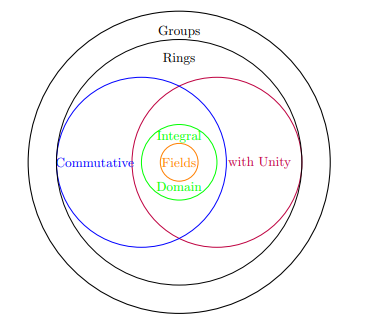
\includegraphics[width=0.5\textwidth]{Figs/algebric_structures.png}
    \caption{Algebraic Structures}
\end{figure}

\subsection{Spaces}

\subsubsection{Vector Space}

A major difference between a field and a vector space is that the operations on a field \( \mathbb{F} \) are
\begin{itemize}
    \item \( +: \mathbb{F} \times \mathbb{F} \to \mathbb{F} \)
    \item \( \times: \mathbb{F} \times \mathbb{F} \to \mathbb{F} \)
\end{itemize}

but the operations on a vector space \( \mathbb{V} \) over a field \( \mathbb{F} \) are
\begin{itemize}
    \item \( +: \mathbb{V} \times \mathbb{V} \to \mathbb{V} \)
    \item \( \cdot: \mathbb{F} \times \mathbb{V} \to \mathbb{V} \)
\end{itemize}

\bigbreak

\begin{definition}{\textbf{Vector Space}} \\
    A vector space over a field \( F \) is a non-empty set \( V \) together with two operations: vector addition \( + \) and scalar multiplication \( \cdot \), satisfying the following axioms for every \( u, v, w \in V \) and \( a, b \in F \):
    \begin{enumerate}
        \item Associativity of vector addition: \( u + (v + w) = (u + v) + w \)
        \item Commutativity of vector addition: \( u + v = v + u \)
        \item Identity element of vector addition: There exists an element \( 0 \in V \), called the \textbf{zero vector}, such that \( v + 0 = v \) for all \( v \in V \).
        \item Inverse elements of vector addition: For every \( v \in V \), there exists an element \( -v \in V \), called the \textbf{additive inverse} of \( v \), such that \( v + (-v) = 0 \).
        \item Compatibility of scalar multiplication with field multiplication: \( a(bv) = (ab)v \)
        \item Identity element of scalar multiplication: \( 1v = v \), where \( 1 \) denotes the multiplicative identity in \( F \).
        \item Distributivity of scalar multiplication with respect to vector addition: \( a(u + v) = au + av \)
        \item Distributivity of scalar multiplication with respect to field addition: \( (a + b)v = av + bv \)
    \end{enumerate}
\end{definition}

\begin{example*}
Examples of vector spaces:
\begin{enumerate}
\item \( \mathbb{R}^n \) is a vector space.
\item The space \( M_{m \times n}(\mathbb{F}) \) of \( m \times n \) matrices over a field \(\mathbb{F}\) is a vector space.
\item The set of all continuous functions over some interval is a vector space.
\item The space of all differentiable functions over a certain interval is a vector space.
\end{enumerate}
\end{example*}

\begin{definition}{\textbf{Homeomorphism (Vector spaces)}} \\
    Let \(V\) and \(W\) be vector spaces over the same field \(F\). A map \( T: V \to W \) is called a \textbf{homomorphism}, 
    or more specifically, a \textbf{linear transformation}, if for all vectors \(u, v \in V\) and any scalar \(c \in F\), the following conditions hold:
    \begin{itemize}
        \item \textbf{Additivity:} \( T(u + v) = T(u) + T(v) \).
        \item \textbf{Homogeneity:} \( T(c \cdot u) = c \cdot T(u) \).
    \end{itemize}
    These conditions ensure that the map \(T\) preserves the vector space structure between \(V\) and \(W\).
\end{definition}


\begin{definition}{\textbf{Complex conjugate}} \\
    The complex conjugate of a complex number \( z = a + bi \) is the number \( \overline{z} = a - bi \).
\end{definition}

\subsubsection{Inner Product Space}

\begin{definition}{\textbf{Inner Product Space}} \\
    An inner product space is a vector space \( V \) over a field \( F \) equipped with an inner product, which is a function that associates each pair of vectors \( u, v \) in \( V \) with a scalar in \( F \), denoted \( \langle u, v \rangle \), and satisfies the following properties for all \( u, v, w \in V \) and \( a \in F \):
    \begin{enumerate}
        \item Linearity in the first argument: \( \langle au + v, w \rangle = a \langle u, w \rangle + \langle v, w \rangle \)
        \item Conjugate symmetry: \( \langle u, v \rangle = \overline{\langle v, u \rangle} \)
        \item Positive-definiteness: \( \langle u, u \rangle \geq 0 \) and \( \langle u, u \rangle = 0 \) if and only if \( u = 0 \)
    \end{enumerate}
\end{definition}

\begin{definition}{\textbf{Hermetian adjoint}} \\
    Let \( V \) be an inner product space over a field \( F \). 
    The Hermetian adjoint of a linear operator \( T: V \to V \) is the unique linear operator \( T^*: V \to V \) such that for all \( u, v \in V \), we have \( \langle Tu, v \rangle = \langle u, T^*v \rangle \).
\end{definition}

A classic exmaple of an inner product space is the \textbf{Euclidean space} \( \mathbb{E}^n \), which is a vector space equipped with 
the inner product \( \langle u, v \rangle = u^T v \).
The geometry of Euclidean space follows the familiar rules of Euclidean geometry, which include notions such as angles, lengths, and the Pythagorean theorem.
It is always complete, meaning that every Cauchy sequence in Euclidean space converges to a point within the space.
Euclidean space can be thought of as the "standard" \( n \)-dimensional space that conforms to our intuitive geometric concepts.



% * * * * * * * * * * * * * * * * * * * * * * * * 
% * * * * * * * * * * * * * * * * * * * * * * * * 
% * * * * * * * * * * * * * * * * * * * * * * * * 
% * * * * * * * * * * * * * * * * * * * * * * * * 
% * * * * * * * * * * * * * * * * * * * * * * * * 
% * * * * * * * * * * * * * * * * * * * * * * * * 
% * * * * * * * * * * * * * * * * * * * * * * * * 
% * * * * * * * * * * * * * * * * * * * * * * * * 
% * * * * * * * * * * * * * * * * * * * * * * * * 
% * * * * * * * * * * * * * * * * * * * * * * * * 
% * * * * * * * * * * * * * * * * * * * * * * * * 
% * * * * * * * * * * * * * * * * * * * * * * * * 
% * * * * * * * * * * * * * * * * * * * * * * * * 
% * * * * * * * * * * * * * * * * * * * * * * * * 
% * * * * * * * * * * * * * * * * * * * * * * * * 
% * * * * * * * * * * * * * * * * * * * * * * * * 
% * * * * * * * * * * * * * * * * * * * * * * * * 
% * * * * * * * * * * * * * * * * * * * * * * * * 
% * * * * * * * * * * * * * * * * * * * * * * * * 

\chapter{Topology and manifolds}

\section{Metric space and complete metric space}

\begin{definition}{\textbf{Metric Space}} \\
    A metric space is a set \( X \) equipped with a metric, which is a function that defines a distance between each pair of elements in \( X \), satisfying the following properties for all \( x, y, z \in X \):
    \begin{enumerate}
        \item Non-negativity: \( d(x, y) \geq 0 \) and \( d(x, y) = 0 \) if and only if \( x = y \)
        \item Symmetry: \( d(x, y) = d(y, x) \)
        \item Triangle inequality: \( d(x, y) + d(y, z) \geq d(x, z) \)
    \end{enumerate}
\end{definition}

\( \textbf{Inner Producy Space vs Metric Space} \)
\begin{itemize}
    \item An inner product space is a vector space equipped with an inner product, which is a function that associates each pair of vectors with a scalar.
    \item A metric space is a set equipped with a metric, which is a function that defines a distance between each pair of elements in the set.
    \item Every inner product space is a metric space, but not every metric space is an inner product space.
        \begin{example*}
            Each inner product space must satisfy the Parallelogram Law, which states that for all \( u, v \) in the space, \( 2\|u\|^2 + 2\|v\|^2 = \|u + v\|^2 + \|u - v\|^2 \).
            A clasic example of a metric space that is not an inner product space is the space of continuous functions on the interval \([0, 1]\) with the metric \( d(f, g) = \max_{x \in [0, 1]} |f(x) - g(x)| \).
        \end{example*}
\end{itemize}

\begin{definition}{ \textbf{Open $\epsilon$-ball} } \\
    Let \( (X, d) \) be a metric space and \( x \in X \). \\
    The open \(\varepsilon\)-ball centered at \( x \) is the set \(  B(x, \varepsilon) = \{ y \in X : d(x, y) < \varepsilon \} \).
\end{definition}

\begin{definition}{ \textbf{Open set} (metric space) } \\
    A subset \( U \) of a metric space \( (X, d) \) is open if for every point \( x \in U \), 
    there exists an open \(\varepsilon\)-ball centered at \( x \) that is contained in \( U \).
\end{definition}

\begin{definition}{\textbf{Convergence of a sequence}} \\
    A sequence \( (x_n) \) in a metric space \( (X, d) \) is said to \emph{converge} to a limit \( a \in X \) if, for every positive real number \( \varepsilon > 0 \),
    there exists a positive integer \( N \) such that for all positive integers \( n \geq N \), \( x_n \in B_{\varepsilon}(a) \).
\end{definition}

\begin{definition}{\textbf{Cauchy Sequence}} \\
    In a metric space \( (X, d) \), a sequence \( \{x_1, x_2, x_3, \ldots\} \) is said to be \emph{Cauchy} if, for every positive real number \( \varepsilon > 0 \),
     there exists a positive integer \( N \) such that for all positive integers \( m, n > N \), the distance
    \[ d(x_m, x_n) < \varepsilon. \]
\end{definition}

\begin{figure}[H]
    \begin{subfigure}{0.5\textwidth}
        \centering
        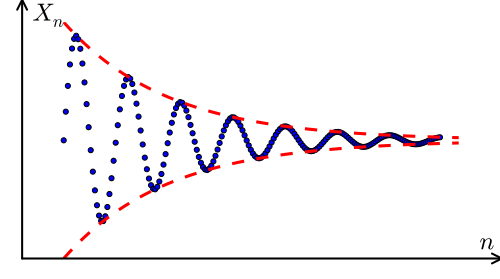
\includegraphics[width=0.45\textwidth]{Figs/Cauchy_sequence_illustration.png}
        \caption{The plot of a Cauchy sequence \( (x_n) \) shown in blue, as \( x_n \) versus \( n \). If the space is complete, then the sequence has a limit.}
    \end{subfigure}
    \hfill
    \begin{subfigure}{0.45\textwidth}
        \centering
        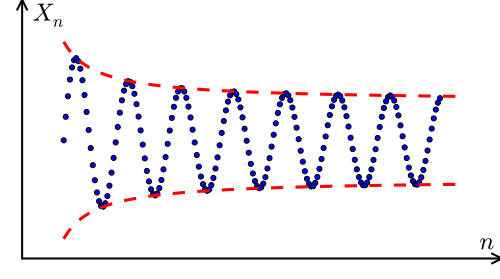
\includegraphics[width=0.5\textwidth]{Figs/Cauchy_sequence_illustration2.png}
        \caption{A sequence that is not Cauchy. The elements of the sequence do not get arbitrarily close to each other as the sequence progresses.}
    \end{subfigure}
    \caption{Cauchy Sequence}
\end{figure}

\begin{definition}{\textbf{Complete Metric Space}} \\
    A metric space is complete if every Cauchy sequence in the space converges to a limit in the space.
\end{definition}

\subsubsection{Hilbert Space}

\begin{definition}{\textbf{Hilbert Space}} \\
    A \emph{Hilbert space} is a complete inner product space. That is, it is an inner product space \( \mathcal{H} \) that 
    is also a complete metric space with respect to the metric induced by its inner product. 
    The metric is given by \( d(x,y) = \sqrt{\langle x-y, x-y \rangle} \) for all \( x, y \in \mathcal{H} \).
\end{definition}
    
A Hilbert space generalizes the notion of Euclidean space to an infinite-dimensional context. 
In a Hilbert space, one can still use concepts like angle, orthogonality, and projection, which are crucial in many areas of mathematics and physics. 
Completeness is a key feature of Hilbert spaces, meaning that every Cauchy sequence in the space converges to a limit within the space. 
    

% * * * * * * * * * * * * * * * * * * * * * * * *
% * * * * * * * * * * * * * * * * * * * * * * * *
% * * * * * * * * * * * * * * * * * * * * * * * *
% * * * * * * * * * * * * * * * * * * * * * * * *
% * * * * * * * * * * * * * * * * * * * * * * * *
% * * * * * * * * * * * * * * * * * * * * * * * *
% * * * * * * * * * * * * * * * * * * * * * * * *


\section{Topological Space}

\begin{definition}{\textbf{Topology}} \\
A topology \( \mathcal{T} \) on a set \( X \) is a collection of subsets of  \( X \) that satisfy the following properties:
\begin{enumerate}
    \item \( \emptyset, X \in \mathcal{T} \).
    \item The intersection of any finite number of sets is in \( \mathcal{T} \) - \\ 
    \( U_1, U_2, \ldots, U_n \in \mathcal{T} \) implies \( \bigcap_{i=1}^n U_i \in \mathcal{T} \).
    \item The union of any number of sets (finite or infinite) is in \( \mathcal{T} \) - \\
    \( U_\alpha \in \mathcal{T} \) for all \( \alpha \) in some index set \( A \) implies \( \bigcup_{\alpha \in A} U_\alpha \in \mathcal{T} \).
\end{enumerate}
\end{definition}

\begin{definition}{\textbf{Topological Space}} \\
A topological space is a pair \( (X, \mathcal{T}) \) consisting of a set \( X \) and a topology \( \mathcal{T} \) on \( X \).
\end{definition}

\begin{example*}
Examples of topological spaces:
\begin{enumerate}
    \item \( X = {1, 2, 3} \) with the topology \( T = \{\varnothing , \{1\}, \{1, 2\}, \{1, 2, 3\} \} \).
    \item Given any set $X$, \textbf{the discrete topology} on $X$ is the power set of $X$ - $\mathcal{T} = P(X)$ and is the largest possible topology on $X$.
    \item \textbf{The indiscrete topology} on $X$ is $\mathcal{T} = \{\emptyset, X\}$ and is the smallest possible topology on $X$ - 
    $\forall \mathcal{T}$, $\{\emptyset, X\} \subseteq \mathcal{T} \subseteq P(X)$.
    \item The real line \( \mathbb{R} \) with the standard topology.
    \item The set of integers \( \mathbb{Z} \) with the discrete topology.
    \item The set of real numbers \( \mathbb{R} \) with the lower limit topology.
\end{enumerate}
\end{example*}

\begin{definition}{\textbf{Open Set (topological space)}} \\
    A subset \( U \) of a topological space \( (X, \mathcal{T}) \) is open if \( U \in \mathcal{T} \).
\end{definition}

% * * * * * * * * * * * * * * * * * * * * * * * *
% * * * * * * * * * * * * * * * * * * * * * * * *
% * * * * * * * * * * * * * * * * * * * * * * * *
% * * * * * * * * * * * * * * * * * * * * * * * *
% * * * * * * * * * * * * * * * * * * * * * * * *
% * * * * * * * * * * * * * * * * * * * * * * * *
% * * * * * * * * * * * * * * * * * * * * * * * *


\section{Interior, exterior, boundary, and accumulation points}

Let \( (X, \mathcal{T}) \) be a topological space , and \( S \subseteq X \) (it can be an open set but it not necessarily has to be).

\begin{definition}{\textbf{Interior point}} \\
    A point \( p \in S \) is an interior point of \( S \) if there exists an open set \( U \) such that \( p \in U \subseteq S \).
\end{definition}

\begin{definition}{\textbf{Exterior point}} \\
    A point \( p \in X \) is an exterior point of \( S \) if there exists an open set \( U \) such that \( p \in U \subseteq X \setminus S \).
\end{definition}

\begin{definition}{\textbf{Boundary point}} \\
    A point \( p \in X \) is a boundary point of \( S \) if for every open set \( U \) containing \( p \), both \( U \cap S \) and \( U \cap (X \setminus S) \) are non-empty.
\end{definition}

\begin{definition}{\textbf{Accumulation (limit) point}} \\
    A point \( p \in X \) is an accumulation point of \( S \) if for every open set \( U \) containing \( p \), the set \( ( U \setminus \{p\} ) \cap S \) is non-empty.
\end{definition}

\begin{figure}[H]
    \begin{subfigure}{0.24\textwidth}
        \centering
        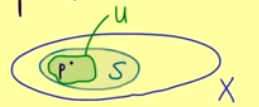
\includegraphics[width=\textwidth]{Figs/interior.png}
        \caption{Interior point}
    \end{subfigure}
    \begin{subfigure}{0.24\textwidth}
        \centering
        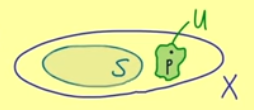
\includegraphics[width=\textwidth]{Figs/exterior.png}
        \caption{Exterior point}
    \end{subfigure}
    \begin{subfigure}{0.24\textwidth}
        \centering
        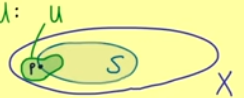
\includegraphics[width=\textwidth]{Figs/boundary.png}
        \caption{Boundary point}
    \end{subfigure}
    \begin{subfigure}{0.24\textwidth}
        \centering
        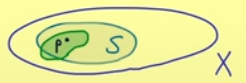
\includegraphics[width=\textwidth]{Figs/accumulation.png}
        \caption{Accumulation point}
    \end{subfigure}
    \caption{Interior, exterior, and boundary points of a set}
\end{figure}


\begin{definition}{\textbf{Interior of a set}} \\
    The interior of a set \( S \), denoted by \( \text{int}(S) \) or \( S^\circ \), is the set of all interior points of \( S \).
    \begin{equation*}
        S^\circ = \{ p \in S : p \text{ is an interior point of } S \}
    \end{equation*}
\end{definition}


\begin{definition}{\textbf{Exterior of a set}} \\
    The exterior of a set \( S \), denoted by \( \text{ext}(S) \), is the set of all exterior points of \( S \).
    \begin{equation*}
        \text{ext}(S) = \{ p \in X : p \text{ is an exterior point of } S \}
    \end{equation*}
\end{definition}

\begin{definition}{\textbf{Boundary of a set}} \\
    The boundary of a set \( S \), denoted by \( \text{bd}(S) \) or \( \partial S \), is the set of all boundary points of \( S \).
    \begin{equation*}
        \partial(S) = \{ p \in X : p \text{ is a boundary point of } S \}
    \end{equation*}
\end{definition}

The boundary of a set \( S \) consists of all points that are either in the interior of \( S \) or in the exterior of \( S \).


\begin{definition}{\textbf{Derived set} (derivative of a set)} \\
    The derived set of a set \( S \), denoted by \( S' \), is the set of all accumulation points of \( S \).
    \begin{equation*}
        S' = \{ p \in X : p \text{ is an accumulation point of } S \}
    \end{equation*}
\end{definition}

\begin{definition}{\textbf{Closure of a set}} \\
    The closure of a set \( S \), denoted by \( \overline{S} \), is the set of all points in \( X \) that are either in \( S \) or are accumulation points of \( S \).
    \begin{equation*}
        \overline{S} = S \cup S'
    \end{equation*}
\end{definition}


\begin{example*}
    X = \( \mathbb{R} \) ,  \( \mathbb{T} = \{ \emptyset, \mathbb{R} \} \cup \{ ( a, \infty ) : a \in \mathbb{R} \} \) is a topology on \( \mathbb{R} \). \\
    S = \( (0, 1) \) is not an open set, and do not have any interior points. \\
    $ X \setminus S = (-\infty, 0] \cup [1, \infty) \Rightarrow  \text{ext}(S) = (1, \infty) \Rightarrow \partial S =  [-\infty, 1)  $.)
    
\end{example*}

% * * * * * * * * * * * * * * * * * * * * * * * *
% * * * * * * * * * * * * * * * * * * * * * * * *
% * * * * * * * * * * * * * * * * * * * * * * * *
% * * * * * * * * * * * * * * * * * * * * * * * *
% * * * * * * * * * * * * * * * * * * * * * * * *
% * * * * * * * * * * * * * * * * * * * * * * * *
% * * * * * * * * * * * * * * * * * * * * * * * *

\section{Hausdorff space}

\begin{definition}{\textbf{Open neighbothood of a point}} \\
    An open neighborhood of a point \( a \) in a topological space \( (X, \mathcal{T}) \) is an open set containing \( a \).
\end{definition}


\begin{definition}{ \textbf{Convergence of a sequence} } \\
    A sequence \( (x_n) \) in a topological space \( (X, \mathcal{T}) \) is said to converge to a limit \( a \in X \) 
    if for every open neighborhood \( U \) of \( a \), there exists a positive integer \( N \) such that for all positive integers \( n \geq N \), \( x_n \in U \).
\end{definition}

Note that there can be multiple limits of a sequence in a topological space, and the limit need not be unique.

\begin{example*}
    X = \( \mathbb{R} \) ,  \( \mathbb{T} = \{ \emptyset, \mathbb{R} \} \cup \{ ( a, \infty ) : a \in \mathbb{R} \} \) is a topology on \( \mathbb{R} \). \\
    \( (a_n)_{n \in \mathbb{N}} = (\frac{1}{n})_{n \in \mathbb{N}} \) converges to 0, but also to any \( a \in (0, \infty) \).
    \begin{itemize}
        \item It converges to 0 - every open neighborhood of 0 looks like \( (a, \infty) \) for some \( a < 0 \) so \( \frac{1}{n} \in (a, \infty) \).
        \item It converges to -1 - every open neighborhood of -1 looks like \( (a, \infty) \) for some \( a < -1 \) so \( \frac{1}{n} \in (a, \infty) \).
        \item The same argument can be made for any \( a \in (-\infty, 0] \).
    \end{itemize}
\end{example*}

\begin{definition}{\textbf{Hausdorff Space}} \\
    A topological space \( (X, \mathcal{T}) \) is a Hausdorff space if for every pair of distinct points \( x, y \in X \), there exist open sets \( U \) and \( V \) such that \( x \in U \), \( y \in V \), and \( U \cap V = \emptyset \).
\end{definition}

\begin{figure}[H]
    \centering
    
\includegraphics[width=0.3\textwidth]{Figs/hausdorff_space.png}
    \caption{Hausdorff space}
\end{figure}

In a Hausdorff space, every pair of distinct points can be separated by disjoint open sets.

% * * * * * * * * * * * * * * * * * * * * * * * *
% * * * * * * * * * * * * * * * * * * * * * * * *
% * * * * * * * * * * * * * * * * * * * * * * * *
% * * * * * * * * * * * * * * * * * * * * * * * *
% * * * * * * * * * * * * * * * * * * * * * * * *
% * * * * * * * * * * * * * * * * * * * * * * * *
% * * * * * * * * * * * * * * * * * * * * * * * *


\section{Quotient space}

\begin{definition}{\textbf{Projective space}} \\
    The projective space \( \mathbf{P}^n (\mathbb{R}) \) is the set of all lines passing through the origin in \( \mathbb{R}^{n+1} \).
    It can be thought of as the space of all one-dimensional subspaces of \( \mathbb{R}^{n+1} \).
\end{definition}

\begin{figure}[H]
    \centering
    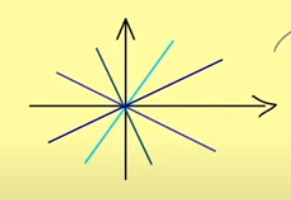
\includegraphics[width=0.3\textwidth]{Figs/projective_space_2d.png}
    \caption{The projective space \( \mathbf{P}^1 \) - all the lines passing through the origin in \( \mathbb{R}^2 \) }
\end{figure}

The directions define a set, and we want to create a topological space for this set.

\begin{definition}{\textbf{Equivalence relation}} \\
    An equivalence relation on a set \( X \) is a relation \( \sim \) that satisfies the following properties for all \( x, y, z \in X \):
    \begin{enumerate}
        \item Reflexivity: \( x \sim x \)
        \item Symmetry: \( x \sim y \) implies \( y \sim x \)
        \item Transitivity: \( x \sim y \) and \( y \sim z \) implies \( x \sim z \)
    \end{enumerate}
\end{definition}

\begin{definition}{\textbf{Equivalence class}} \\
    Let \( X \) be a set and \( \sim \) be an equivalence relation on \( X \). \\
    The equivalence class of \( x \) with respect to \( \sim \) is
    \begin{equation*}
        [x]_\sim = \{ y \in X : y \sim x \}
    \end{equation*}
\end{definition}

\begin{definition}{\textbf{Quotient set}} \\
    Let \( X \) be a set and \( \sim \) be an equivalence relation on \( X \). \\
    The quotient set \( X / \sim \) is defined as 
    \begin{equation*}
        X/\sim \quad = \{ [x]_\sim : x \in X \}
    \end{equation*}
\end{definition}

\begin{definition}{\textbf{Quotient map (Canonical projection)}} \\
    Let \( X \) be a set and \( \sim \) be an equivalence relation on \( X \). \\
    The canonical projection is a function:
    \begin{equation*}
        q: X \to X/\sim \quad \text{such that} \quad q(x) = [x]_\sim
    \end{equation*}
\end{definition}

\begin{definition}{\textbf{Quotient Topology}} \\
    Let \( X , \mathcal{T} \) be a topological space, \( \sim \) be an equivalence relation on \( X \) and \( q: X \to X/\sim \) be the canonical projection. \\
    The quotient topology \( \hat{\mathcal{T}} \) on \( X/\sim \) is defined as
    \begin{equation*}
        \hat{\mathcal{T}} = \{ U \subseteq X/\sim \quad : q^{-1}(U) \in \mathcal{T} \}
    \end{equation*}
\end{definition}

\begin{figure}[H]
    \centering
    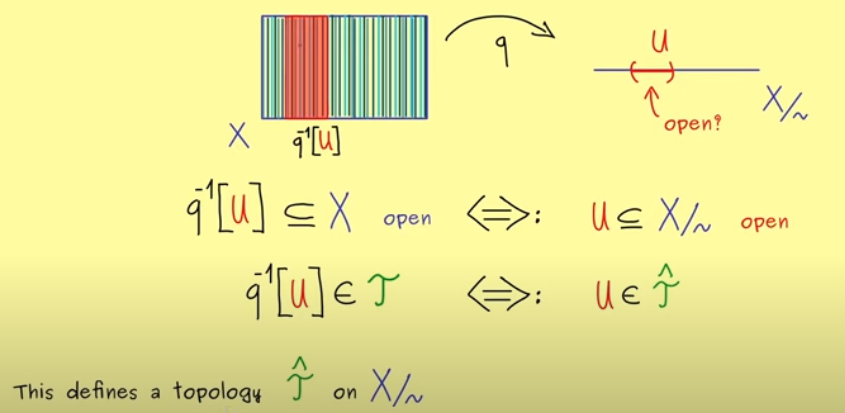
\includegraphics[width=0.8\textwidth]{Figs/quotient_topology.png}
    \caption{Quotient Topology}
\end{figure}

\begin{example*} A classic example of a quotient space is the \textbf{mobius strip}, which is constructed by taking a rectangular strip of paper, 
    giving one end a half-twist, and then gluing the two ends together. The mobius strip is a non-orientable surface, 
    meaning that it does not have a consistent notion of "left" and "right" across the entire surface. 
    The mobius strip is a quotient space of a square, where the opposite edges of the square are identified in a specific way.
    Formally, 
    \begin{align*}
        X = [0, 1] \times (-1, 1) \quad \text{and} \quad &\sim \text{ is the equivalence relation that identifies the points} \\
        (0, y) &\sim (1, -y) \quad \text{for all} \quad y \in (-1, 1).
    \end{align*}
\end{example*}

\begin{figure}[H]
    \centering
    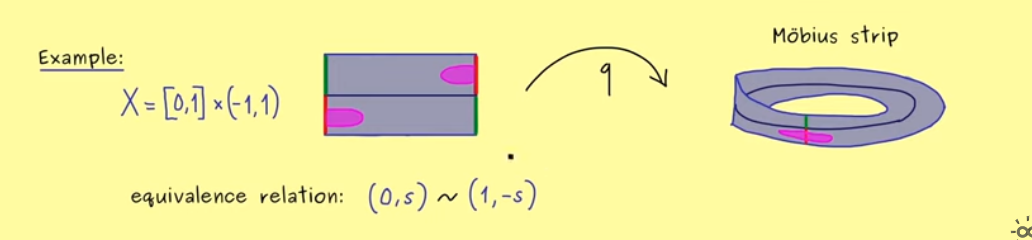
\includegraphics[width=0.8\textwidth]{Figs/mobius_strip.png}
    \caption{Mobius Strip}
\end{figure}

% * * * * * * * * * * * * * * * * * * * * * * * *
% * * * * * * * * * * * * * * * * * * * * * * * *
% * * * * * * * * * * * * * * * * * * * * * * * *
% * * * * * * * * * * * * * * * * * * * * * * * *
% * * * * * * * * * * * * * * * * * * * * * * * *
% * * * * * * * * * * * * * * * * * * * * * * * *
% * * * * * * * * * * * * * * * * * * * * * * * *


\section{Projective Space}

So far we have seen the transition from topological space to quotient space:
\begin{equation*}
    (X, \mathcal{T}) \to (X/\sim, \hat{\mathcal{T}})
\end{equation*}

Recall that the projective space \( \mathbf{P}^n (\mathbb{R}) \) is the set of all lines passing through the origin in \( \mathbb{R}^{n+1} \).

\begin{definition}{\textbf{Sphere}} \\
    The sphere \( S^n \) is the set of all points in \( \mathbb{R}^{n+1} \) that are at a fixed distance of 1 from the origin.
    \begin{equation*}
        S^n = \{ x \in \mathbb{R}^{n+1} : \|x\|_2 = 1 \}
    \end{equation*}
\end{definition}

\begin{definition}{\textbf{The Projective Space as quotient space}} \\
    The projective space \( \mathbf{P}^n (\mathbb{R}) \) can be constructed as a quotient space of the sphere \( S^n \) by identifying antipodal points.
    \begin{equation*}
        \mathbf{P}^n (\mathbb{R}) = S^n / \sim
    \end{equation*}
    where the equivalence relation \( \sim \) is defined as
    \begin{equation*}
        x \sim y \quad \text{if} \quad x = y \quad \text{or} \quad x = -y
    \end{equation*}
\end{definition}

\begin{figure}[H]
    \centering
    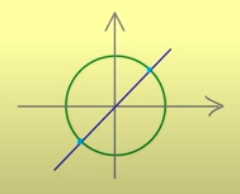
\includegraphics[width=0.3\textwidth]{Figs/projective_space.png}
    \caption{Projective Space as a quotient space}
\end{figure}

The sphere \( S^n \) is a hausdorff space, and the projective space \( \mathbf{P}^n (\mathbb{R}) \) is also a hausdorff space.
But in general, the quotient space of a hausdorff space is not necessarily a hausdorff space.
Take \( [x]_\sim, [y]_\sim \in \mathbf{P}^n (\mathbb{R}) \) such that \( [x]_\sim \neq [y]_\sim \Rightarrow x \neq y \) and \( x \neq -y \) .

\begin{figure}[H]
    \begin{subfigure}{\textwidth}
        \centering
        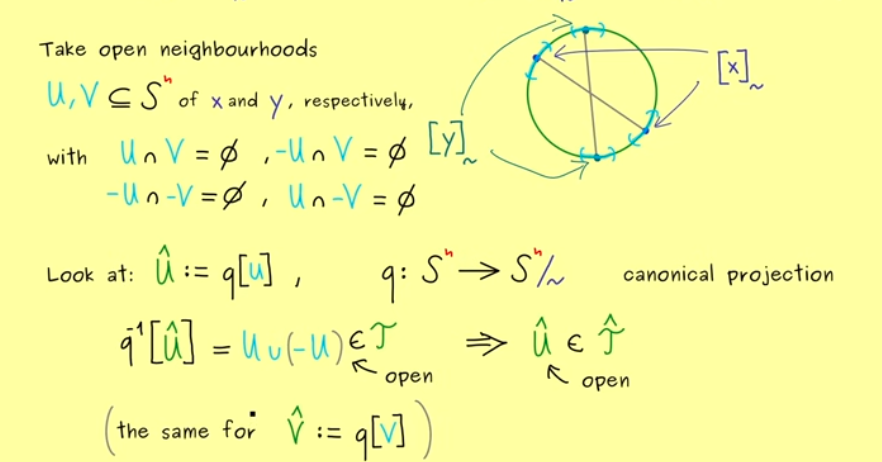
\includegraphics[width=\textwidth]{Figs/projective_space_is_hausdorff.png}
    \end{subfigure}
    \begin{subfigure}{\textwidth}
        \centering
        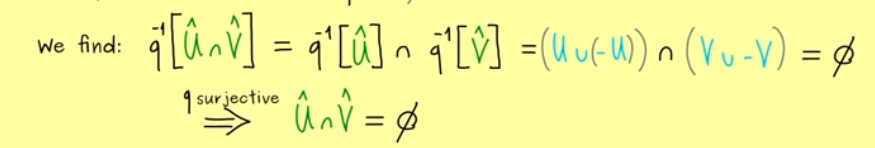
\includegraphics[width=\textwidth]{Figs/projective_space_is_hausdorff2.png}
    \end{subfigure}
    \caption{Projective Space as a hausdorff space}
\end{figure}

% * * * * * * * * * * * * * * * * * * * * * * * *
% * * * * * * * * * * * * * * * * * * * * * * * *
% * * * * * * * * * * * * * * * * * * * * * * * *
% * * * * * * * * * * * * * * * * * * * * * * * *
% * * * * * * * * * * * * * * * * * * * * * * * *
% * * * * * * * * * * * * * * * * * * * * * * * *
% * * * * * * * * * * * * * * * * * * * * * * * *

\section{Second Countable Space}

\begin{definition}{\textbf{Basis}} \\
    A basis for a topological space \( (X, \mathcal{T}) \) is a collection \( \mathcal{B} \subseteq \mathcal{T} \) of open sets
     such that every open set in \( \mathcal{T} \) can be written as a union of sets in \( \mathcal{B} \).
\end{definition}

\begin{examples*} of basis:
    \begin{itemize}
        \item \( \mathcal{B} = \mathcal{T} \) is a basis for \( \mathcal{T} \).
        \item If \( \mathcal{T} \) is discrete, then \( \mathcal{B} = \{ \{ x \} : x \in X \} \) is a basis for \( \mathcal{T} \).
        \item Let \( (X, \mathcal{T}) \) be a topological space induced by a metric space \( (X, d) \). \\
            Then \( \mathcal{B} = \{ B_\varepsilon(x) : x \in X, \varepsilon > 0 \} \) is a basis for \( \mathcal{T} \).
        \item \( \mathbb{R}^n \) with the standard topology (defined by the Euclidean metric) has a basis of open balls.
            Then \( \mathcal{B} = \{ B_{\varepsilon}(x) : x \in \mathbb{Q}^n, \varepsilon \in \mathbb{Q}, \varepsilon > 0 \} \) is a basis for \( \mathcal{T} \).
            Eventhought the space is uncountable, the basis has a countable number of elements.
    \end{itemize}
\end{examples*}

\begin{definition}{\textbf{Second Countable Space}} \\
    A topological space \( (X, \mathcal{T}) \) is second countable if there exists a countable basis for \( \mathcal{T} \).
\end{definition}


% * * * * * * * * * * * * * * * * * * * * * * * *
% * * * * * * * * * * * * * * * * * * * * * * * *
% * * * * * * * * * * * * * * * * * * * * * * * *
% * * * * * * * * * * * * * * * * * * * * * * * *
% * * * * * * * * * * * * * * * * * * * * * * * *
% * * * * * * * * * * * * * * * * * * * * * * * *
% * * * * * * * * * * * * * * * * * * * * * * * *

\section{Continuity}

Recall the definition of continuity of a function in $R^n$:
\begin{definition*}{\textbf{Continuity of a function}} \\
    A function \( f: \mathbb{R}^n \to \mathbb{R} \) is continuous at a point \( x \in \mathbb{R}^n \) 
    if for every \( \varepsilon > 0 \), there exists \( \delta > 0 \) such that for all \( y \in \mathbb{R}^n \) with
     \( \| x - y \|_2 < \delta \), we have \( \| f(x) - f(y) \|_2 < \varepsilon \).
\end{definition*}

or equivalently, in term of sequences:
\begin{definition*}{\textbf{Continuity of a function (sequence definition)}} \\
    A function \( f: \mathbb{R}^n \to \mathbb{R} \) is continuous at a point \( x \in \mathbb{R}^n \) 
    if for every sequence \( (x_k) \) in \( \mathbb{R}^n \) such that \( x_k \to x \), we have \( f(x_k) \to f(x) \).
\end{definition*}

Now, we extend the definition of continuity to topological spaces.

\begin{definition}{\textbf{Continuity of a function at a point (topological space)}} \\
    Let \( (X, \mathcal{T}_X) \) and \( (Y, \mathcal{T}_Y) \) be topological spaces. \\
    A function \( f: X \to Y \) is continuous at a point \( x \in X \) if for every neighborhood \( V \) of \( f(x) \) in \( Y \),
    there exists a neighborhood \( U \) of \( x \) in \( X \) such that \( f(U) \subseteq V \).
\end{definition}

\begin{figure}[H]
    \centering
    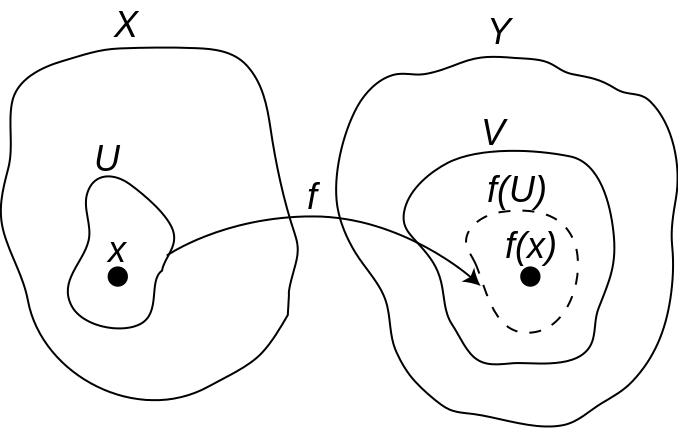
\includegraphics[width=0.4\textwidth]{Figs/continuity_topology.png}
    \caption{Continuity of a function at a point} 
\end{figure}


\begin{corollary}{\textbf{Continuity of a function (topological space)}} \\
    Let \( (X, \mathcal{T}_X) \) and \( (Y, \mathcal{T}_Y) \) be topological spaces. \\
    A function \( f: X \to Y \) is continuous if for every open set \( U \in \mathcal{T}_Y \), \( f^{-1}(U) \in \mathcal{T}_X \) \\
    (the preimage of an open set is open).
\end{corollary}

\begin{figure}[H]
    \centering
    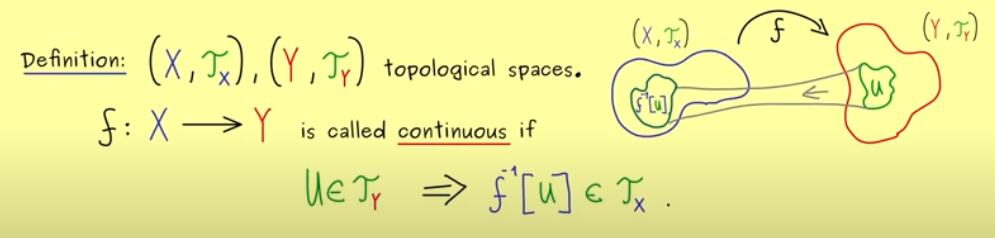
\includegraphics[width=\textwidth]{Figs/continuity.png}
    \caption{Continuity of a function}    
\end{figure}

or equivalently, in term of sequences:
\begin{definition}{\textbf{Sequentially continuous function (topological space)}} \\
    Let \( (X, \mathcal{T}_X) \) and \( (Y, \mathcal{T}_Y) \) be topological spaces. \\
    A function \( f: X \to Y \) is sequentially continuous if for every \( x \in X \) and every sequence 
    \( (x_n)_{n \in \mathbb{N}} \subseteq X \) such that \( x_n \to x \), \( (f(x_n))_{n \in \mathbb{N}} \subseteq Y \) convergent 
    with \( (f(x_n))_{n \in \mathbb{N}} \to f(x) \).
\end{definition}

\begin{figure}[H]
    \centering
    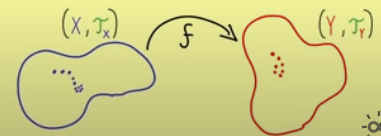
\includegraphics[width=0.4\textwidth]{Figs/sequentially_continues_function.png}
    \caption{Sequentially continuous function}
\end{figure}


\begin{definition}{\textbf{Homeomorphism} (NOT homomorphism)} \\ 
    A function \( f: X \to Y \) between topological spaces \( (X, \mathcal{T}_X) \) and \( (Y, \mathcal{T}_Y) \) is a homeomorphism if
    \begin{enumerate}
        \item \( f \) is bijective (both injective and surjective - one-to-one and onto).
        \item \( f : X \to Y \) is continuous.
        \item \( f^{-1} : Y \to X \) is continuous.
    \end{enumerate}
\end{definition}

\begin{examples*} of continuous maps
    \begin{itemize}
        \item The indiscrete topology on \( X \) and \( Y \) - every function is continuous. \\
            e.g., \( \forall f: X \to Y \) , \( \mathcal{T}_X = \{ \emptyset, X \} \) and \( \mathcal{T}_Y = \{ \emptyset, Y \} \), 
            then \( f \) is continuous since the preimage of any open set in \( Y \) is either \( \emptyset \) or \( X \).

        \item The discrete topology on \( X \) and \( Y \) - every function is continuous. \\
            e.g., \( \forall f: X \to Y \) , \( \mathcal{T}_X = P(X) \) and \( \mathcal{T}_Y = P(Y) \), 
            then \( f \) is continuous since the preimage of any open set in \( Y \) must be a subset of \( X \).

        \item The quotient map \( q: X \to X/\sim \) is continuous. \\
            Let \( (X, \mathcal{T}) \) be a topological space and \( \sim \) be an equivalence relation on \( X \). \\
            Then the quotient map \( q: X \to X/\sim \) is continuous.
            \begin{proof}
                Let \( U \in \mathcal{T}_{X/\sim} \) be an open set in \( X/\sim \). \\
                Then \( q^{-1}(U) \in \mathcal{T}_X \) is an open set in \( X \) by definition of the quotient topology. 
                The same argument holds for the other direction.
            \end{proof}
    \end{itemize}
\end{examples*}


% * * * * * * * * * * * * * * * * * * * * * * * *
% * * * * * * * * * * * * * * * * * * * * * * * *
% * * * * * * * * * * * * * * * * * * * * * * * *
% * * * * * * * * * * * * * * * * * * * * * * * *
% * * * * * * * * * * * * * * * * * * * * * * * *
% * * * * * * * * * * * * * * * * * * * * * * * *
% * * * * * * * * * * * * * * * * * * * * * * * *


% * * * * * * * * * * * * * * * * * * * * * * * *
% * * * * * * * * * * * * * * * * * * * * * * * *
% * * * * * * * * * * * * * * * * * * * * * * * *
% * * * * * * * * * * * * * * * * * * * * * * * *
% * * * * * * * * * * * * * * * * * * * * * * * *
% * * * * * * * * * * * * * * * * * * * * * * * *
% * * * * * * * * * * * * * * * * * * * * * * * *


% * * * * * * * * * * * * * * * * * * * * * * * * 
% * * * * * * * * * * * * * * * * * * * * * * * * 
% * * * * * * * * * * * * * * * * * * * * * * * * 
% * * * * * * * * * * * * * * * * * * * * * * * * 
% * * * * * * * * * * * * * * * * * * * * * * * * 
% * * * * * * * * * * * * * * * * * * * * * * * * 
% * * * * * * * * * * * * * * * * * * * * * * * * 
% * * * * * * * * * * * * * * * * * * * * * * * * 
% * * * * * * * * * * * * * * * * * * * * * * * * 
% * * * * * * * * * * * * * * * * * * * * * * * * 
% * * * * * * * * * * * * * * * * * * * * * * * * 
% * * * * * * * * * * * * * * * * * * * * * * * * 
% * * * * * * * * * * * * * * * * * * * * * * * * 
% * * * * * * * * * * * * * * * * * * * * * * * * 
% * * * * * * * * * * * * * * * * * * * * * * * * 
% * * * * * * * * * * * * * * * * * * * * * * * * 
% * * * * * * * * * * * * * * * * * * * * * * * * 
% * * * * * * * * * * * * * * * * * * * * * * * * 
% * * * * * * * * * * * * * * * * * * * * * * * * 

\chapter{Convexity and Optimization}

\section{Important subsets of $\mathbb{R}^n$}

\begin{definition}{Open set} \\
A set $S \subseteq \mathbb{R}^n$ is open if for all $x \in S$, there exists $\epsilon > 0$ such that $B(x, \epsilon) \subseteq S$.
\end{definition}

\begin{definition}{Closed set} \\
A set $S \subseteq \mathbb{R}^n$ is closed if its complement is open.
\end{definition}

\begin{definition}{Interior point} \\
A point $x \in S$ is an interior point of $S$ if there exists $\epsilon > 0$ such that $B(x, \epsilon) \subseteq S$.
\end{definition}

\begin{corollary}{Open set characterization} \\
A set $S \subseteq \mathbb{R}^n$ is open if and only if every point in $S$ is an interior point of $S$.
\end{corollary}

\begin{definition}{Boundary point} \\
A point $x \in S$ is a boundary point of $S$ if for all $\epsilon > 0$, $B(x, \epsilon) \cap S \neq \emptyset$ and $B(x, \epsilon) \cap S^c \neq \emptyset$.
\end{definition}

\begin{definition}{Half-space} \\
A half-space in $\mathbb{R}^n$ is a set of the form $\{x \in \mathbb{R}^n : a^T x \leq b\}$ for some $a \in \mathbb{R}^n$ and $b \in \mathbb{R}$.
\end{definition}

\begin{definition}{Hyperplane} \\
A hyperplane in $\mathbb{R}^n$ is a set of the form $\{x \in \mathbb{R}^n : a^T x = b\}$ for some $a \in \mathbb{R}^n$ and $b \in \mathbb{R}$.
\end{definition}

\begin{definition}{Polyhedron (Polyhedra)} \\
A polyhedron in $\mathbb{R}^n$ is a set of the form $\{x \in \mathbb{R}^n : Ax \leq b\}$ for some $A \in \mathbb{R}^{m \times n}$ and $b \in \mathbb{R}^m$.
Equivalently, a polyhedron is the intersection of finitely many half-spaces.
\end{definition}

\begin{definition}{Polytope} \\
A polytope in $\mathbb{R}^n$ is a bounded polyhedron - i.e., there exists $r > 0$ such that $\forall x \in \{x \in \mathbb{R}^n : Ax \leq b\} \implies ||x|| \leq r$.
Equivalently, a polytope is the convex hull of finitely many points.
\end{definition}

\begin{figure}[H]
    \centering
    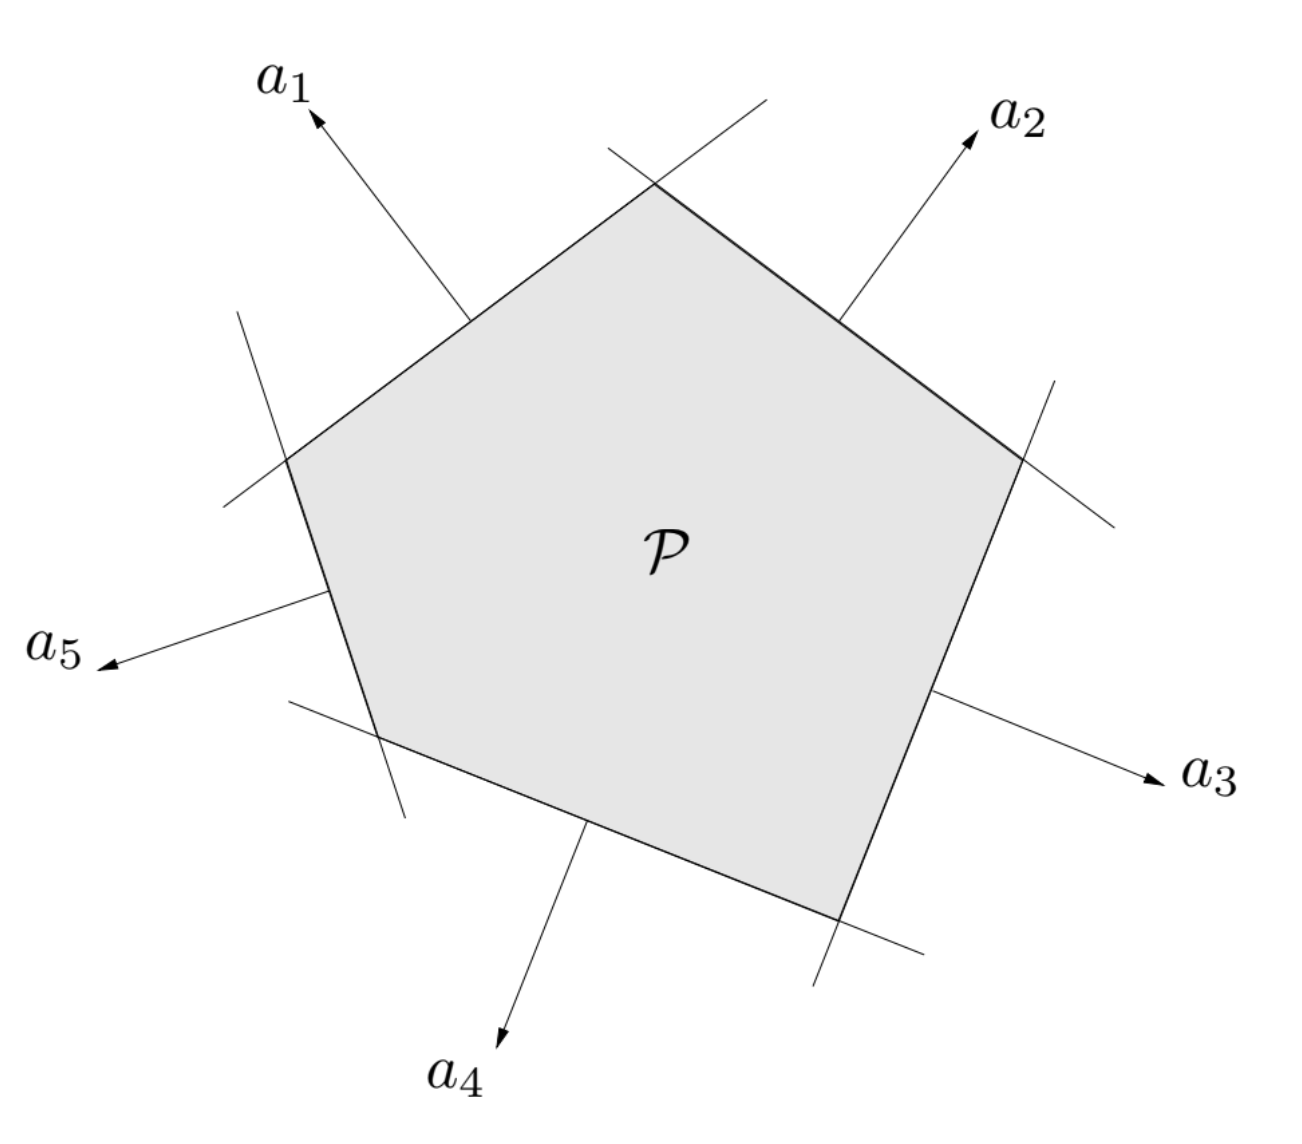
\includegraphics[width=0.3\textwidth]{Figs/polyhedron.png}
    \caption{Polytope}
\end{figure}

\begin{definition}{Convex set} \\
    A set $S \subseteq \mathbb{R}^n$ is convex if for all $x,y \in S$ and $\lambda \in [0,1]$, we have $\lambda t + (1- \lambda)y \in S$.
\end{definition}    

\begin{figure}[H]
    \centering
    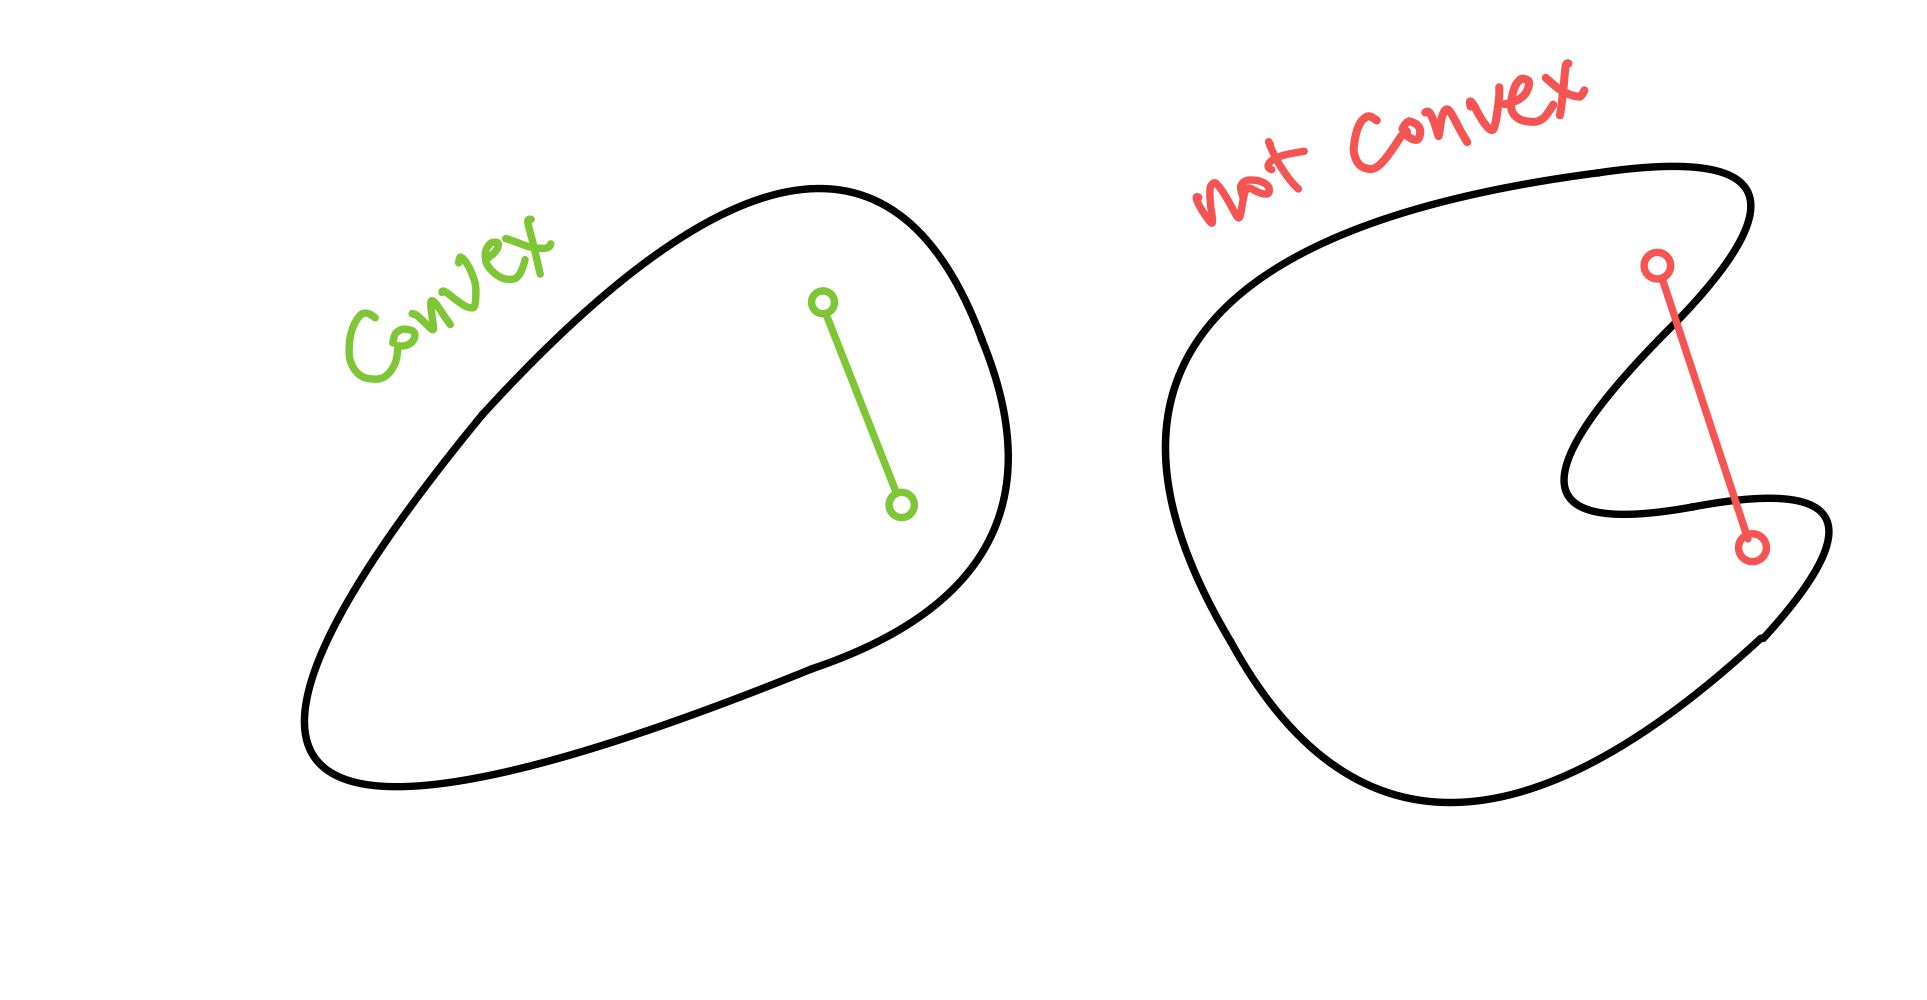
\includegraphics[width=0.5\textwidth]{Figs/convex_set.png}
    \caption{Convex set}
\end{figure}

\begin{definition}{Convex hull} \\
The convex hull of a set $S \subseteq \mathbb{R}^n$ is the smallest convex set that contains $S$.
\end{definition}


\begin{definition}{Conic combination} \\
A point $x \in \mathbb{R}^n$ is a conic combination of $y_1, \ldots, y_k \in \mathbb{R}^n$ 
if there exist $\lambda_1, \ldots, \lambda_k \geq 0$ such that $x = \sum_{i=1}^k \lambda_i y_i$.    
\end{definition}

\begin{definition}{Conic hull} \\
The conic hull of a finite set $S \subseteq \mathbb{R}^n$ is the set of all conic combinations of points in $S$.
\end{definition}


\begin{definition}{Convex cone} \\
A set $S \subseteq \mathbb{R}^n$ is a convex cone if for all $x \in S$ and $\lambda \geq 0$, we have $\lambda x \in S$.
\end{definition}

\begin{figure}[H]
    \begin{subfigure}{0.5\textwidth}
        \centering
        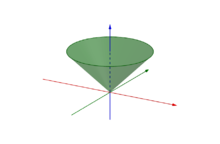
\includegraphics[width=\linewidth]{Figs/circular-pyramid.png}
        \caption{Convex cone that is not a conic hull of finitely many generators.}
    \end{subfigure}
    \begin{subfigure}{0.5\textwidth}
        \centering
        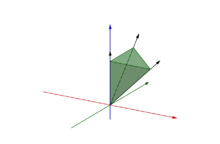
\includegraphics[width=\linewidth]{Figs/polyhedral_cone.png}
        \caption{Convex cone genrated by the conic combination of three black vectors (conic hull).}
    \end{subfigure}
\end{figure}

\begin{definition}{Normal cone} \\
The normal cone to a set $S$ at a point $x$ is defined as
\begin{equation}
    N_S(x) = \{ v \in \mathbb{R}^n : \langle v, y-x \rangle \leq 0 \text{ for all } y \in S \}
\end{equation}
\end{definition}

\begin{definition}{Tangent cone} \\
The tangent cone to a set $S$ at a point $x$ is defined as
\begin{equation}
    T_S(x) = \{ v \in \mathbb{R}^n : \lim_{t \rightarrow 0^+} \frac{x + tv - x}{t} \in S \}
\end{equation}
\end{definition}

\begin{figure}[H]
    \centering
    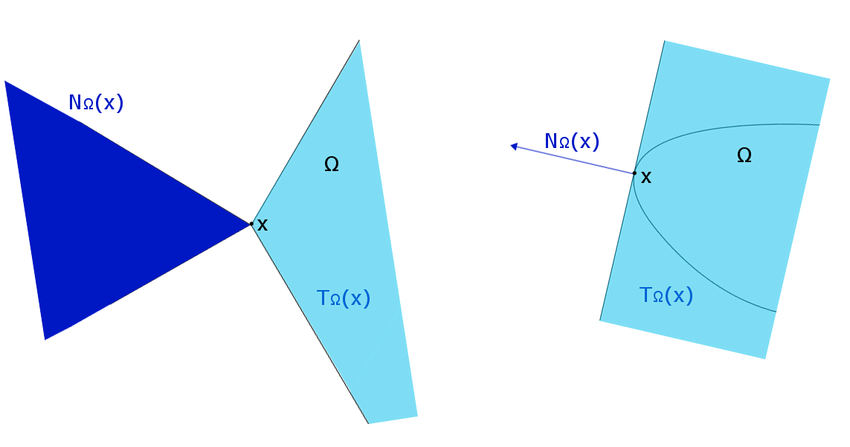
\includegraphics[width=0.5\textwidth]{Figs/normal-cones.png}
    \caption{Normal and tangent cones}
\end{figure}

\begin{theorem}{Normal cone of polyhedron} \\
The normal cone to a polyhedron $S = \{x \in \mathbb{R}^n : \forall j \in [m] \quad a_j \cdot x \leq b_j\}$ at a point $x$ is given by
\begin{equation}
    N_S(x) = \{ \sum_{j} \lambda_j a_j : \lambda_j \geq 0  \text{ and }  a_j \cdot x = b_j \}
\end{equation}
    
\end{theorem}


% * * * * * * * * * * * * * * * * * * * * * * * *
% * * * * * * * * * * * * * * * * * * * * * * * *
% * * * * * * * * * * * * * * * * * * * * * * * *
% * * * * * * * * * * * * * * * * * * * * * * * *
% * * * * * * * * * * * * * * * * * * * * * * * *
% * * * * * * * * * * * * * * * * * * * * * * * *
% * * * * * * * * * * * * * * * * * * * * * * * *


\section{Definitions and Fundamental Theorems}



\begin{definition} (Convex function): A function $f : S \rightarrow \mathbb{R}$ defined on a convex set $S$ is convex if, for all $x, y \in S$ and $\lambda \in [0,1]$, 
\[ f(\lambda x + (1-\lambda)y) \leq \lambda f(x) + (1-\lambda) f(y). \]
\end{definition}

\begin{figure}[H]
    \centering
    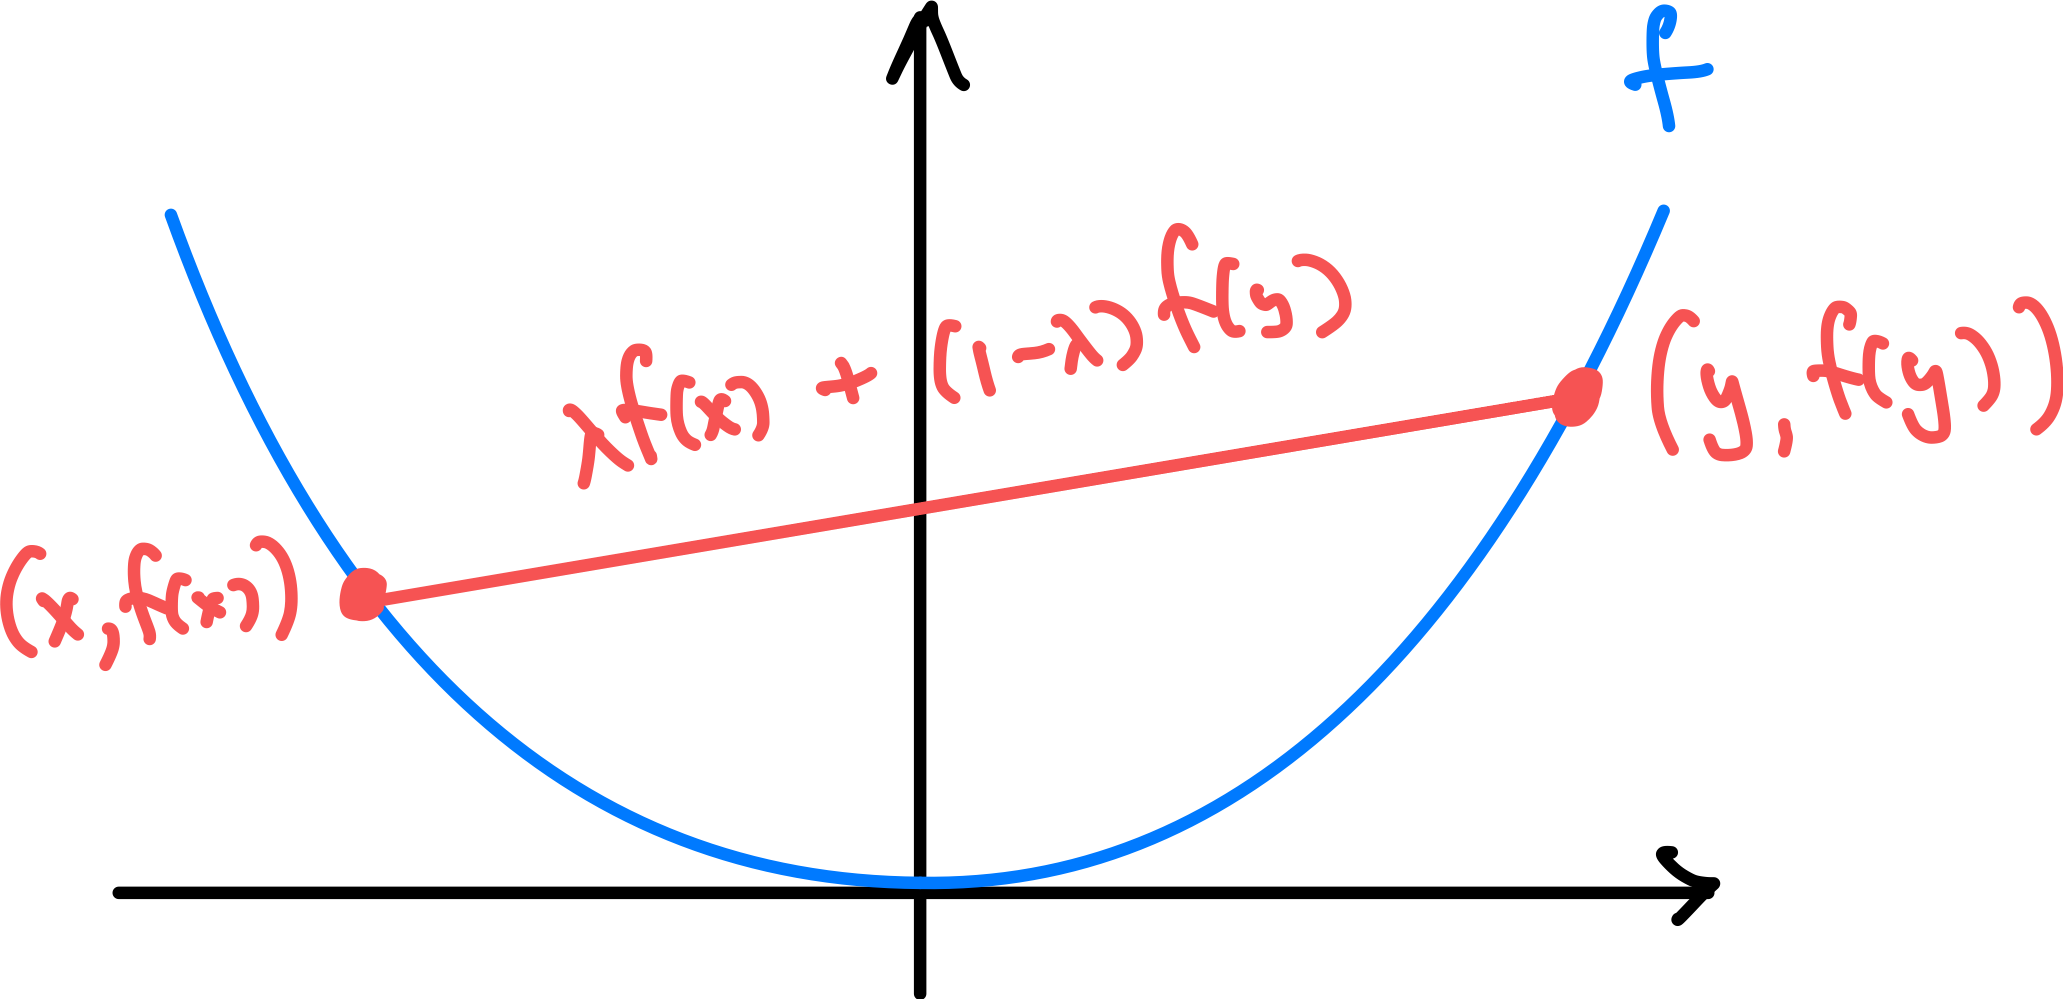
\includegraphics[width=0.5\textwidth]{Figs/convex_function.png}
    \caption{Convex function}
\end{figure}

\begin{theorem} (Characterization via epigraph): A function $f : S \to \mathbb{R}$ is convex if and only if its epigraph $\{(x,t) \in S \times \mathbb{R} : f(x) \leq t\}$ is a convex set.
\end{theorem}

\begin{figure}[H]
    \centering
    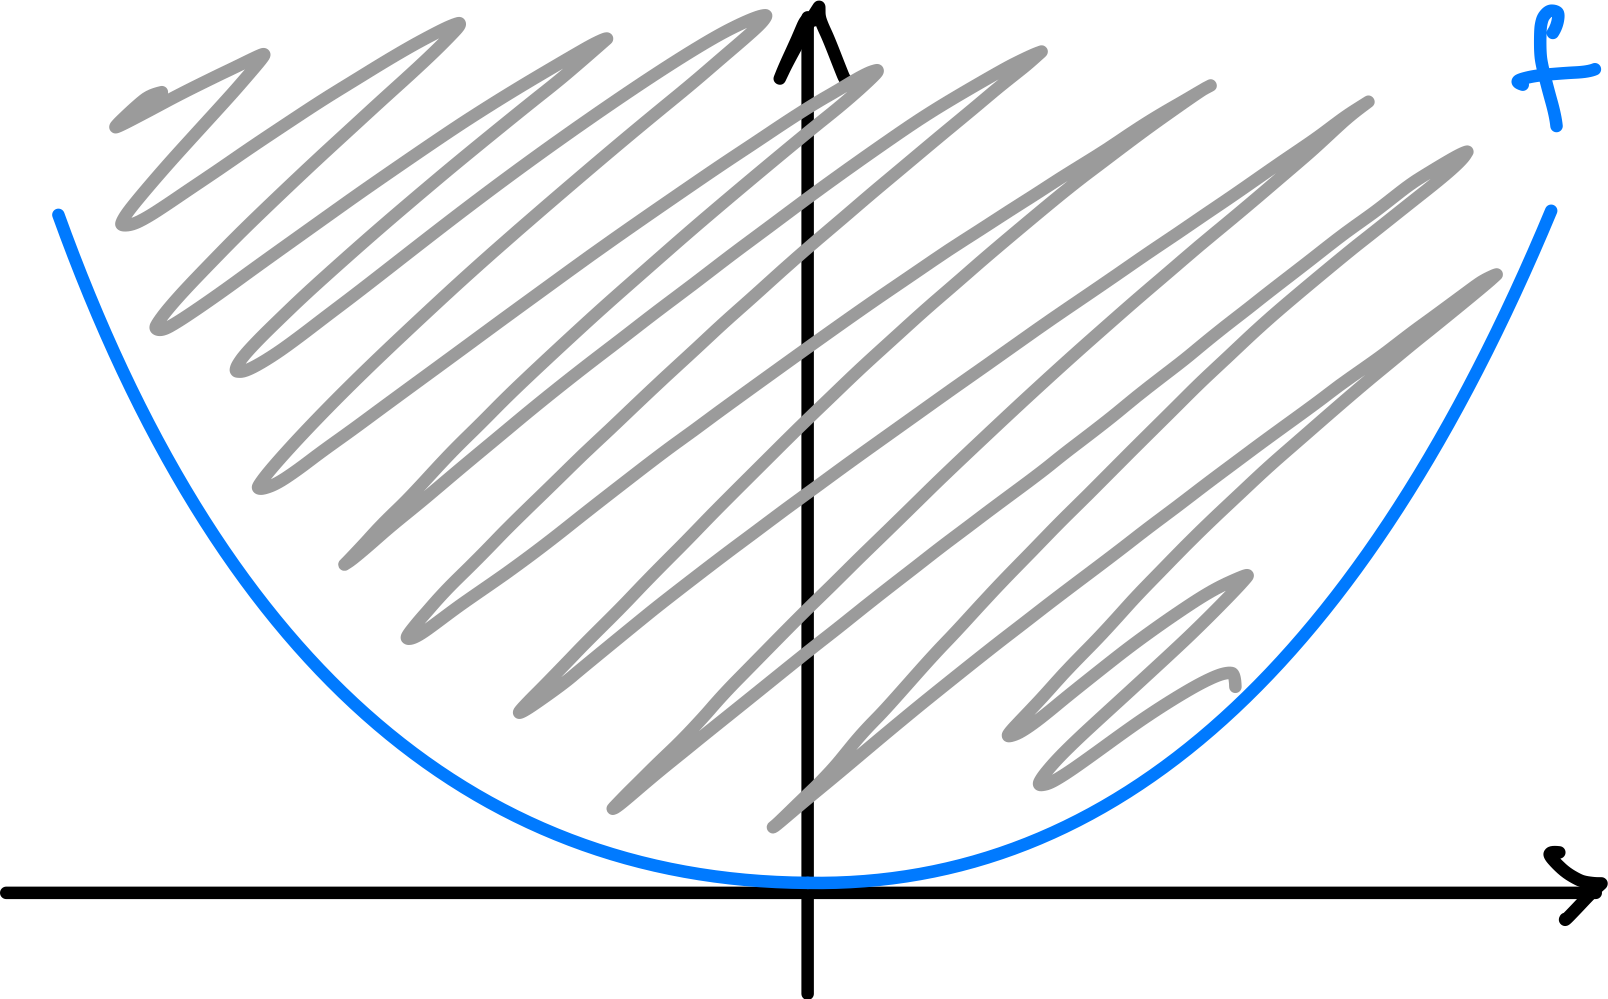
\includegraphics[width=0.3\textwidth]{Figs/epigraph_of_convex_function.png}
    \caption{Epigraph of a convex function}
\end{figure}


\begin{claim} (Convexity of sublevel sets): If $f : S \to \mathbb{R}$ is convex, then the sublevel set $S_t = \{ x \in S : f(x) \leq t\}$ is convex for any $t \in \mathbb{R}$.
\end{claim}

\section{Inequalities and Characterizations}

\begin{theorem}(Jensen's inequality): If $f$ is a convex function, then for any $x_1, x_2, \ldots, x_n \in S$ and any non-negative weights $\alpha_i$ such that $\sum_{i=1}^n \alpha_i = 1$,
\[ f\left(\sum_{i=1}^n \alpha_i x_i\right) \leq \sum_{i=1}^n \alpha_i f(x_i). \]
\end{theorem}


\begin{theorem}(First-order characterization, aka “the gradient inequality”): If $f$ is a differentiable convex function on an open set $S$, then for all $x, y \in S$,
\[ f(y) \geq f(x) + \nabla f(x)^\top (y - x). \]
\end{theorem}

\begin{figure}[H]
    \centering
    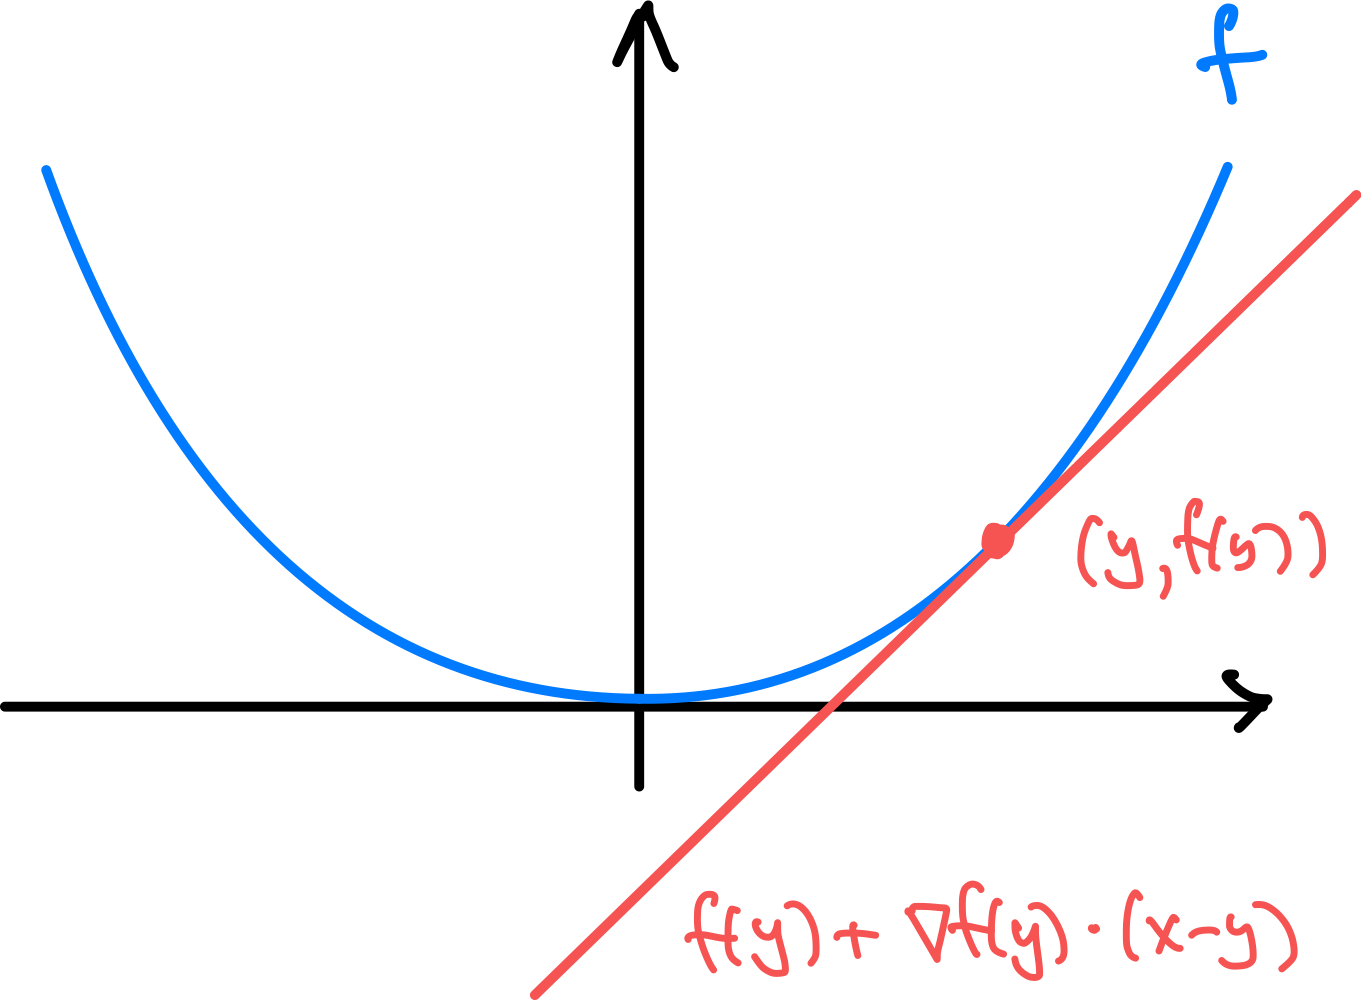
\includegraphics[width=0.3\textwidth]{Figs/first_order_characterization_of_convexity.png}
    \caption{First-order characterization of convexity}
\end{figure}

\begin{definition}{Bergman divergence (distance)} \\
The Bergman divergence between two points $x, y \in \mathbb{R}^n$ is defined as
\begin{equation}
    D_f(x,y) = f(x) - f(y) - \nabla f(y)^\top (x-y)
\end{equation}
\end{definition}


\begin{theorem} (Jensen’s inequality, generalized for expectation): If $f$ is a convex function and $X$ is a random variable over $S$, then
\[ f(\mathbb{E}[X]) \leq \mathbb{E}[f(X)]. \]
\end{theorem}


\begin{theorem} (Second-order characterization of convexity): A twice differentiable function $f$ is convex on an open set $S$ if and only if the Hessian matrix of $f$ is positive semidefinite at every point in $S$.
\end{theorem}

\section{Optimization and Projection}

\begin{definition} (Convex optimization): The problem of minimizing a convex function over a convex set.
\end{definition}

\begin{theorem} (Optimality conditions, unconstrained): If $f$ is convex and differentiable, \\
     $x^*$ is a local minimum of $f$ $\Leftrightarrow$ $x^*$ is a global minimum of $f$ $\Leftrightarrow$  $\nabla f(x^*) = 0$.
\end{theorem}

\begin{theorem} (Optimality conditions, constrained): If $f$ is differentiable and $C$ is a convex set,
     $x^*$ is a local minimum of $f$ on $C$ if and only if $\langle \nabla f(x^*), x - x^* \rangle \geq 0$ for all $x \in C$.
\end{theorem}

\begin{figure}[H]
    \centering
    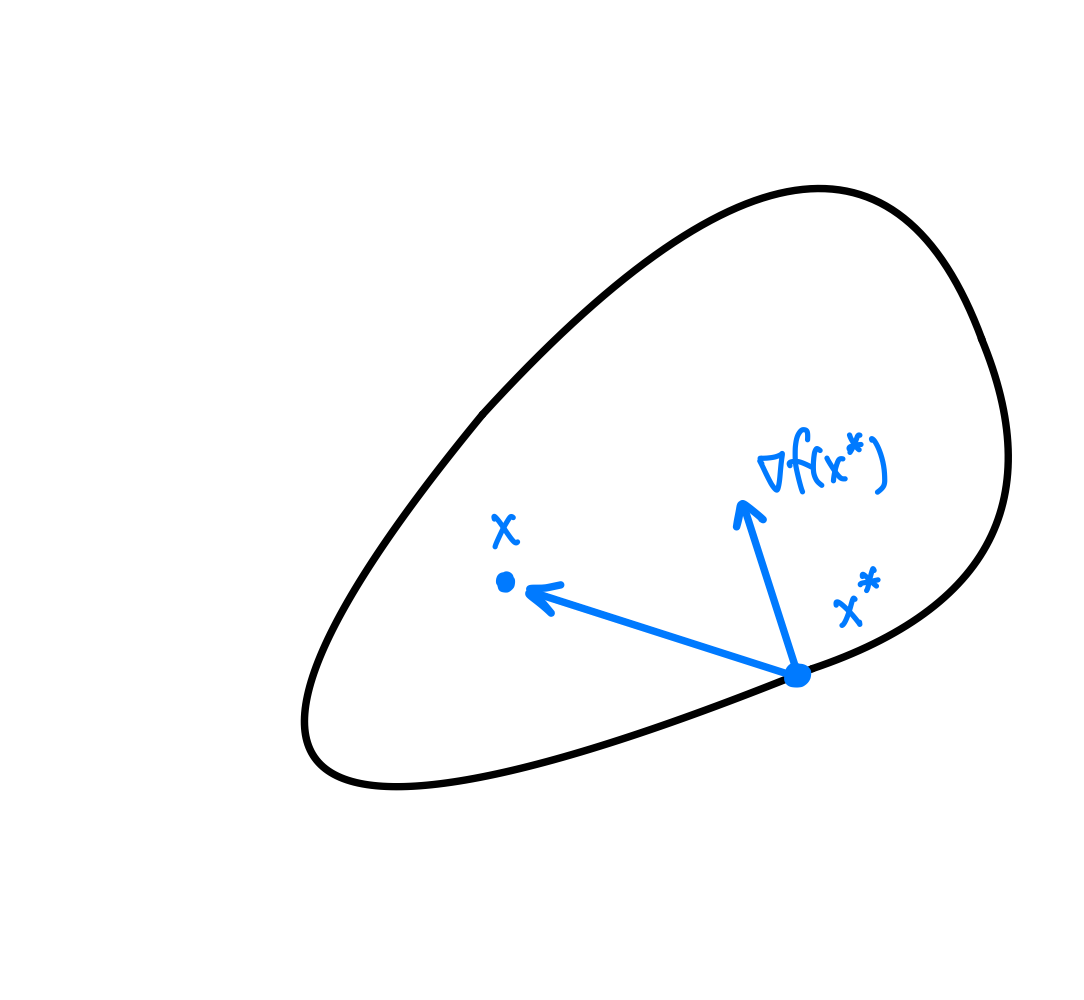
\includegraphics[width=0.5\textwidth]{Figs/optimality_condition_constrained.png}
    \caption{Optimality conditions, constrained}
\end{figure}


\begin{corollary}{Optimality conditions, constrained (alternative)} \\
If $f$ is differentiable and $C$ is a convex set, then $x^*$ is a local minimum of $f$ on $C$ if and only if $-\nabla f(x^*) \in N_C(x^*)$.
\end{corollary}

\begin{definition} (Projection): The projection of a point $x$ onto a convex set $S$ is defined as $\Pi_S(x) = \arg\min_{y \in S} \|y-x\|$.
\end{definition}

\begin{figure}[H]
    \centering
    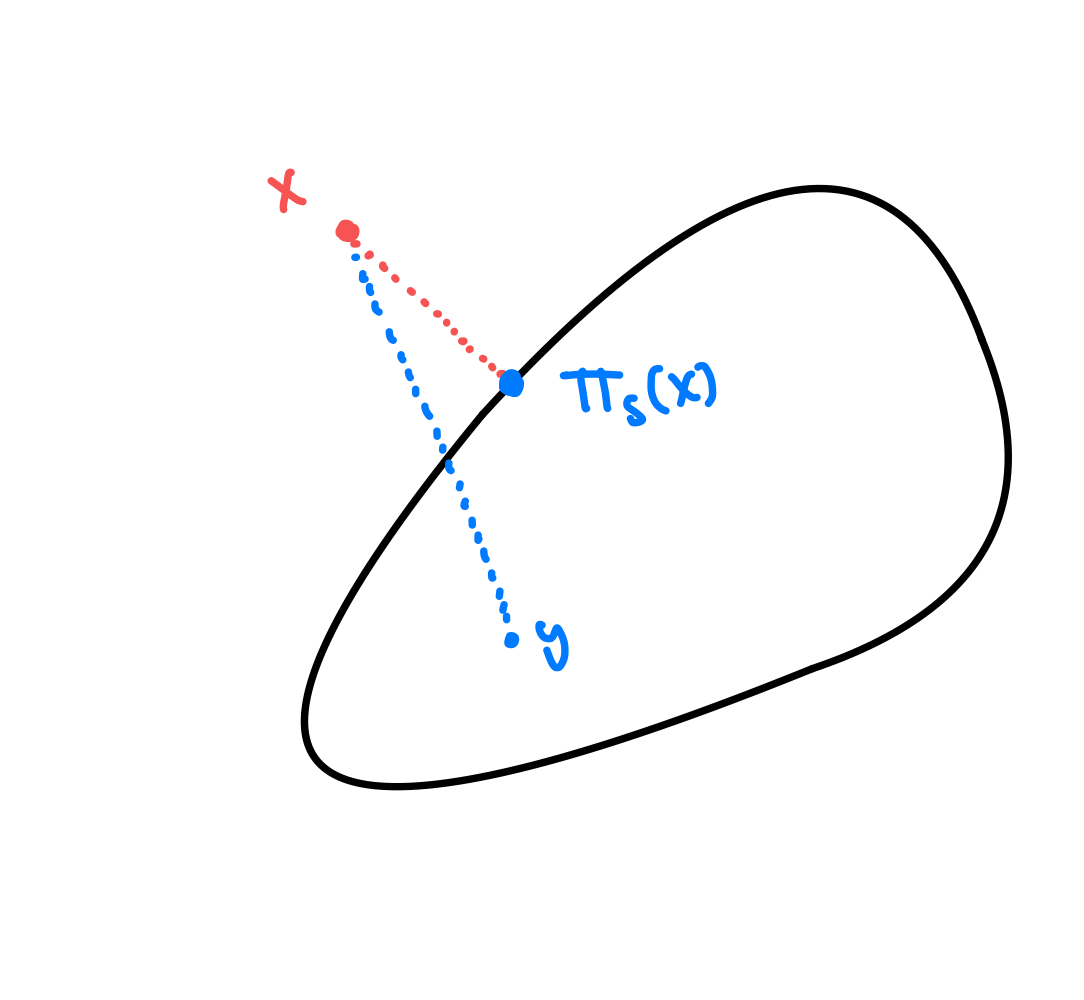
\includegraphics[width=0.3\textwidth]{Figs/projection.png}
    \caption{Projection}
\end{figure}


\begin{theorem} {Generalized cosine theorem} \\
    Let \( S \subseteq \mathbb{R}^d \) be convex and \( x \in \mathbb{R}^d \). Then the projection \( \Pi_S[x] \) is unique and satisfies:
    \begin{equation}
    \| x - \Pi_S[x] \|^2 + \| \Pi_S[x] - y \|^2 \leq \| x - y \|^2, \quad \forall y \in S.
    \end{equation}
    In particular:
    \begin{equation}
    \| \Pi_S[x] - y \| \leq \| x - y \|, \quad \forall y \in S.
    \end{equation}
\end{theorem}


% * * * * * * * * * * * * * * * * * * * * * * * *
% * * * * * * * * * * * * * * * * * * * * * * * *
% * * * * * * * * * * * * * * * * * * * * * * * *
% * * * * * * * * * * * * * * * * * * * * * * * *
% * * * * * * * * * * * * * * * * * * * * * * * *
% * * * * * * * * * * * * * * * * * * * * * * * *
% * * * * * * * * * * * * * * * * * * * * * * * *


\section{Properties of Convex Functions}

\begin{definition}{L - Lipschitz continuous} \\
A function $f: S \rightarrow \mathbb{R}$ is L-Lipschitz continuous if for all $x, y \in S$,
\begin{equation}
    |f(x) - f(y)| \leq L ||x-y||
\end{equation}    
\end{definition}

\begin{theorem}{Convexity and Lipschitz continuity} \\
If $f$ is convex, differentiable and L-Lipschitz continuous, then $||\nabla f(x)|| \leq L$ for all $x \in S$. 
\end{theorem}

\begin{definition} {Smooth function} \\
    A differentiable function \( f \) is \(\beta\)-smooth over \( S \subseteq \text{dom} f \) if for all \( x, y \in S \):
    \[-\frac{\beta}{2} \|y - x\|^2 \leq f(y) - f(x) - \nabla f(x) \cdot (y - x) \leq \frac{\beta}{2} \|y - x\|^2.\]
\end{definition}


\begin{figure}[H]
    \centering
    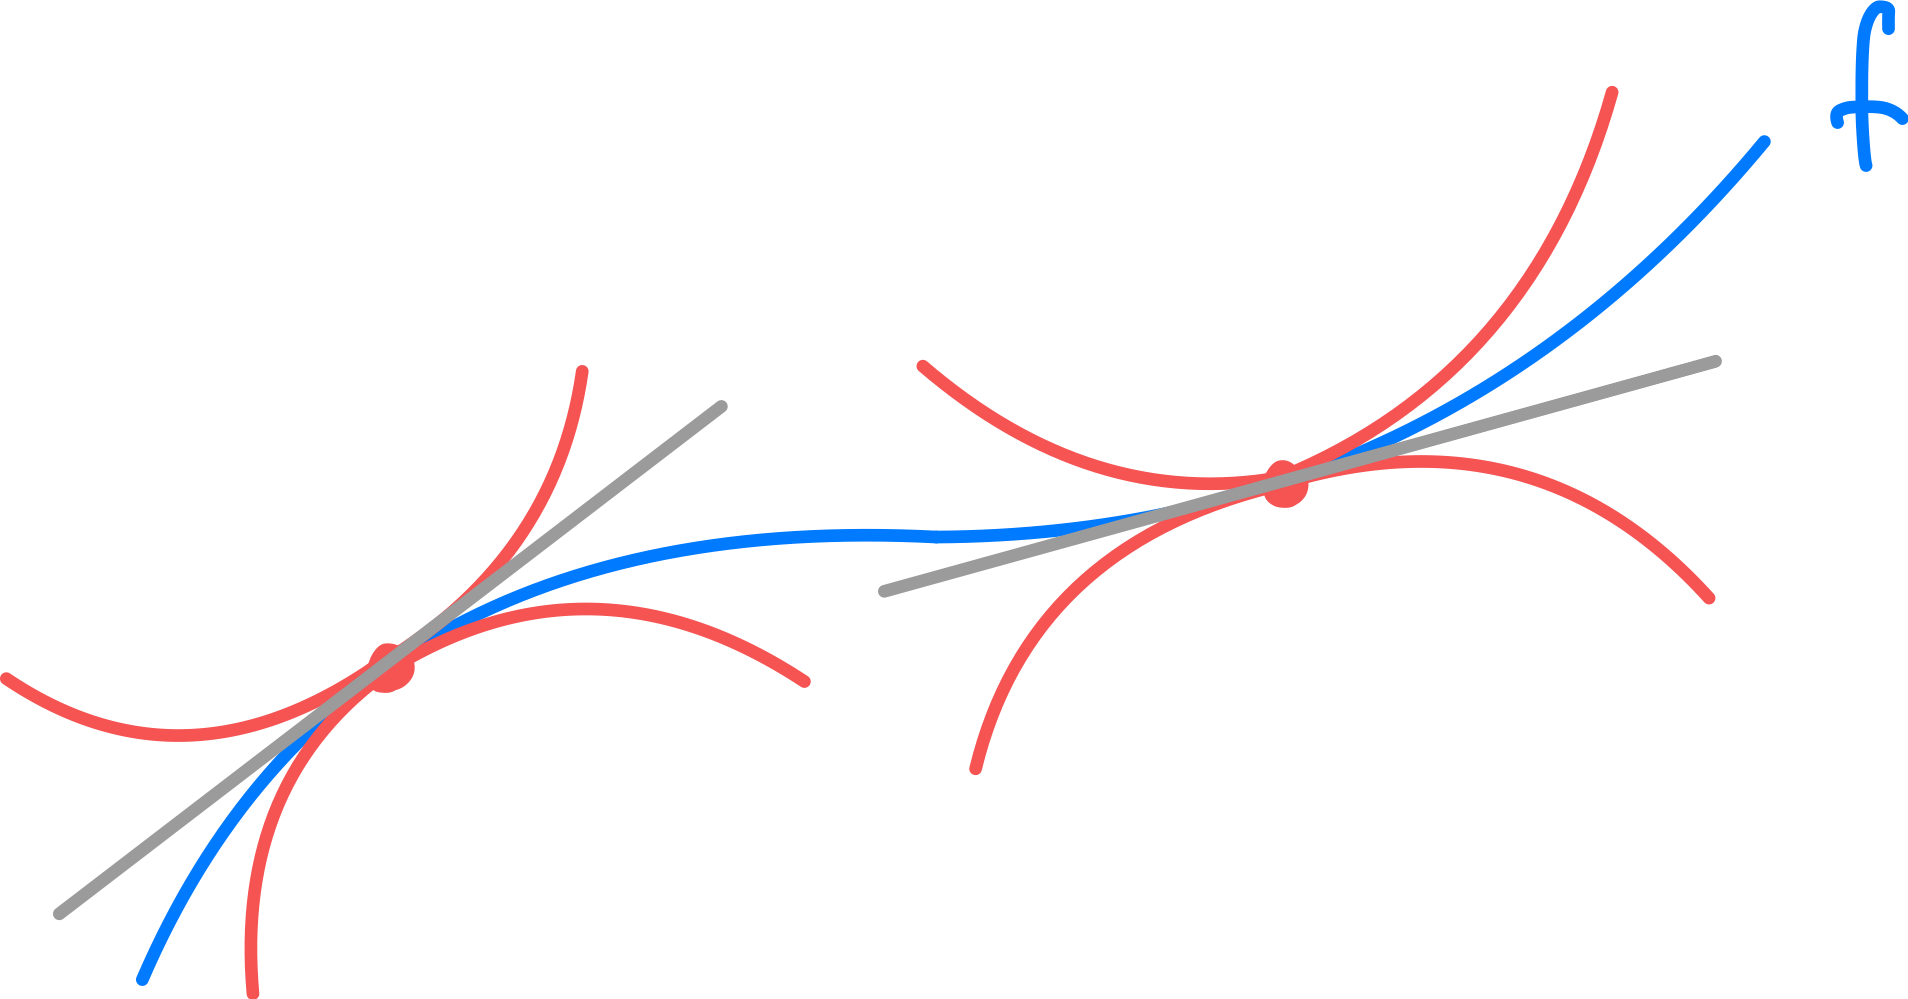
\includegraphics[width=0.7\textwidth]{Figs/beta_smooth_function.png}
    \caption{Smooth function}
\end{figure}


\begin{theorem} {Lipschitz gradient interpretation } \\
Let \( f \) be differentiable and let \( S \subseteq \text{dom} f \) be convex and closed. Suppose that
\[\|\nabla f(x) - \nabla f(y)\| \leq \beta \|x - y\|, \quad \forall x, y \in S.\]
Then \( f \) is \(\beta\)-smooth over \( S \).
\end{theorem}

\begin{theorem} {Second-order characterization of smoothness} \\
Let \( f \) be \( C^2 \) and let \( S \subseteq \text{dom} f \) be convex and closed. Then \( f \) is \(\beta\)-smooth over \( S \) if and only if
\[-\beta I \preceq \nabla^2 f(x) \preceq \beta I, \quad \forall x \in S.\]
\end{theorem}


\begin {lemma} {The Descent Lemma} \\
Let \( f : \mathbb{R}^d \rightarrow \mathbb{R} \) be \(\beta\)-smooth, and let \( x \in \mathbb{R}^d \).
\end{lemma}

\begin{itemize}
    \item For \( \eta \leq \frac{1}{\beta} \), \( x^{+} = x - \eta \nabla f(x) \), we have
    \[ f(x^{+}) - f(x) \leq -\frac{\eta}{2} \|\nabla f(x)\|^2. \]
    \item For \( x^{*} \in \text{arg\,min}_x f(x) \), we have
    \[ \frac{1}{2\beta} \|\nabla f(x)\|^2 \leq f(x) - f(x^{*}). \]
\end{itemize}

\textbf{Basic Facts}:
\begin{itemize}
    \item An affine function \( f : \mathbb{R}^d \rightarrow \mathbb{R}, f(x) = a^\top x + b \), is 0-smooth.
    \item A quadratic function \( f : \mathbb{R}^d \rightarrow \mathbb{R}, f(x) = \frac{1}{2} x^\top A x + b^\top x + c \), is \( \lambda_{\text{max}}(A) \)-smooth.
    \item A linear combination of smooth functions is smooth with an appropriate parameter.
    \item A convex combination of \(\beta\)-smooth functions is \(\beta\)-smooth.
\end{itemize}


\begin{definition} {Strong convexity} \\
A function \( f \) is \(\alpha\)-strongly convex (for \(\alpha \geq 0\)) over a convex and closed set \( S \subseteq \text{dom} f \) if for any \( x \in S \), there exists \( g_x \in \partial f(x) \) such that:
\[
\forall y \in S, \quad f(y) \geq f(x) + g_x \cdot (y - x) + \frac{\alpha}{2} \|y - x\|^2.
\]
In particular, a differentiable \( f \) is \(\alpha\)-strongly convex over \( S \) if for any \( x \in S \),
\[
\forall y \in S, \quad f(y) \geq f(x) + \nabla f(x) \cdot (y - x) + \frac{\alpha}{2} \|y - x\|^2.
\]
\end{definition}

\begin{figure}[H]
    \centering
    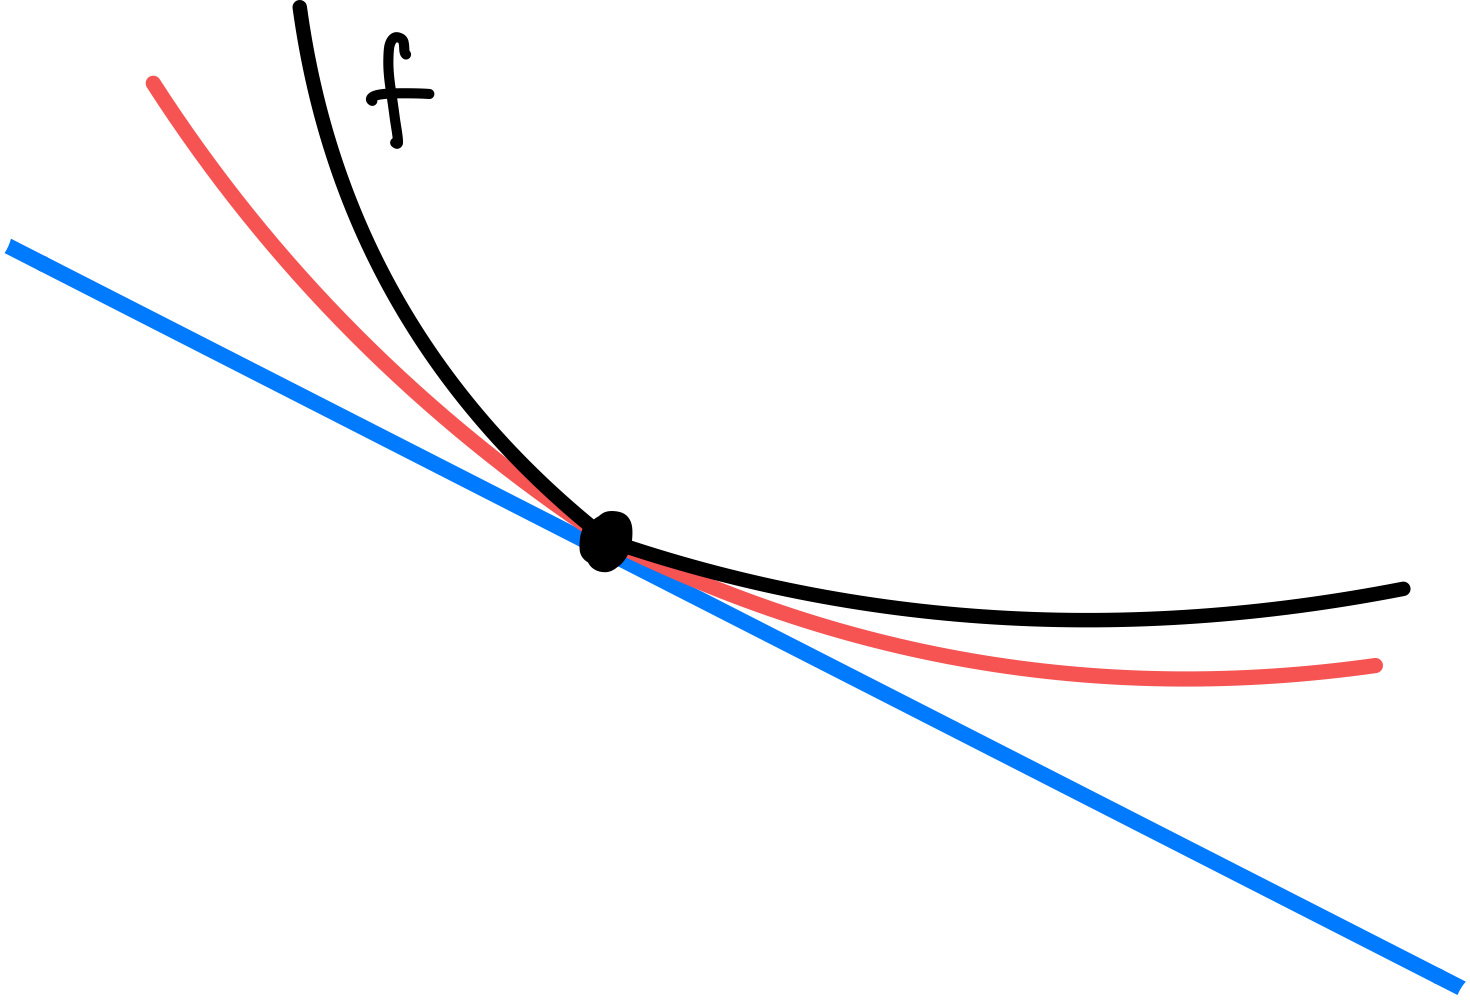
\includegraphics[width=0.5\textwidth]{Figs/strongly_convex.png}
    \caption{Strongly convex function}
\end{figure}

\begin{theorem} { Strong convexity, second-order characterization}\\
Let \( f \) be \( C^2 \) and let \( S \subseteq \text{dom} f \) be convex and closed. Then \( f \) is \(\alpha\)-strongly convex over \( S \) if and only if
\[
\forall x \in S, \quad \nabla^2 f(x) \succeq \alpha I.
\]
\end{theorem}


\begin{theorem} {Usage of strong convexity } \\
If a differentiable \( f \) is \(\alpha\)-strongly convex over a convex and closed \( S \subseteq \text{dom} f \) with a minimum at \( x^* \in S \), then
\[
\forall x \in S, \quad \frac{\alpha}{2} \|x - x^*\|^2 \leq f(x) - f(x^*) \leq \frac{1}{2\alpha} \|\nabla f(x)\|^2.
\]
In particular, the minimum of a strongly convex function is unique.
\end{theorem}


% * * * * * * * * * * * * * * * * * * * * * * * *
% * * * * * * * * * * * * * * * * * * * * * * * *
% * * * * * * * * * * * * * * * * * * * * * * * *
% * * * * * * * * * * * * * * * * * * * * * * * *
% * * * * * * * * * * * * * * * * * * * * * * * *
% * * * * * * * * * * * * * * * * * * * * * * * *
% * * * * * * * * * * * * * * * * * * * * * * * *


\section{Important Inequalities}

\begin{theorem}{$1 + x \leq e^x$} \\
For all $x \in \mathbb{R}$, we have $1 + x \leq e^x$.    
\end{theorem}

\begin{proof}
Let $f(x) = e^x - 1 - x$. Then $f'(x) = e^x - 1$ and $f''(x) = e^x > 0$. Thus, $f$ is convex and $f(0) = 0$. Therefore, $f(x) \geq 0$ for all $x \in \mathbb{R}$.
\end{proof}

\begin{figure}[H]
    \centering
    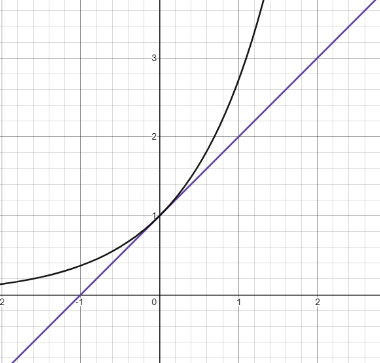
\includegraphics[width=0.3\textwidth]{Figs/1+x_leq_e^x.png}
    \caption{$1 + x \leq e^x$}
\end{figure}


% * * * * * * * * * * * * * * * * * * * * * * * * 
% * * * * * * * * * * * * * * * * * * * * * * * * 
% * * * * * * * * * * * * * * * * * * * * * * * * 
% * * * * * * * * * * * * * * * * * * * * * * * * 
% * * * * * * * * * * * * * * * * * * * * * * * * 
% * * * * * * * * * * * * * * * * * * * * * * * * 
% * * * * * * * * * * * * * * * * * * * * * * * * 
% * * * * * * * * * * * * * * * * * * * * * * * * 
% * * * * * * * * * * * * * * * * * * * * * * * * 
% * * * * * * * * * * * * * * * * * * * * * * * * 
% * * * * * * * * * * * * * * * * * * * * * * * * 
% * * * * * * * * * * * * * * * * * * * * * * * * 
% * * * * * * * * * * * * * * * * * * * * * * * * 
% * * * * * * * * * * * * * * * * * * * * * * * * 
% * * * * * * * * * * * * * * * * * * * * * * * * 
% * * * * * * * * * * * * * * * * * * * * * * * * 
% * * * * * * * * * * * * * * * * * * * * * * * * 
% * * * * * * * * * * * * * * * * * * * * * * * * 
% * * * * * * * * * * * * * * * * * * * * * * * * 



\chapter{The First Miracle: Robustness}

Let f be a convex function, and let $x^*$ be a minimizer of f. 

\section{Gradient Descent}
\begin{definition}{Gradient Descent} \\
    \begin{equation}
       x_{t+1} = x_t - \eta \nabla f(x_t) 
    \end{equation}
\end{definition}

It holds that:
\begin{equation}
    f(x^*) \geq f(x_t) + \nabla f(x_t) \cdot (x^* - x_t)
\end{equation}

\begin{equation}
    0 \leq f(x_t) - f(x^*) \leq \nabla f(x_t) \cdot (x_t - x^*) 
\end{equation}

\subsection{Analysis of the Gradient Descent Algorithm}

\begin{align*}
    \|a\|^2  &= \|b\|^2 + \|a - b\|^2   \\ 
    \|b\|^2 &= \|a\|^2 - \|a - b\|^2 = \|a\|^2 - ( \|a\|^2 - 2a \cdot b + \|b\|^2  ) = 2 a \cdot b - \|b\|^2
\end{align*}
Then we have:
\begin{align*}
    \| x^* - x_t \|^2 - \| x^* - x_{t+1} \|^2 &= - 2 \eta (x^* - x_t) \cdot \nabla f(x_t) - \eta^2 \| \nabla f(x_t) \|^2 \\
    &= 2 \eta (x_t - x^*) \cdot \nabla f(x_t) - \eta^2 \| \nabla f(x_t) \|^2 \\
    &\geq  2 ( f(x_t) - f(x^*) ) - \eta^2 L^2
\end{align*}

Where the last inequality follows from the convexity and the Lipschitz continuity of $f$. 

\begin{figure}[H]
    \centering
    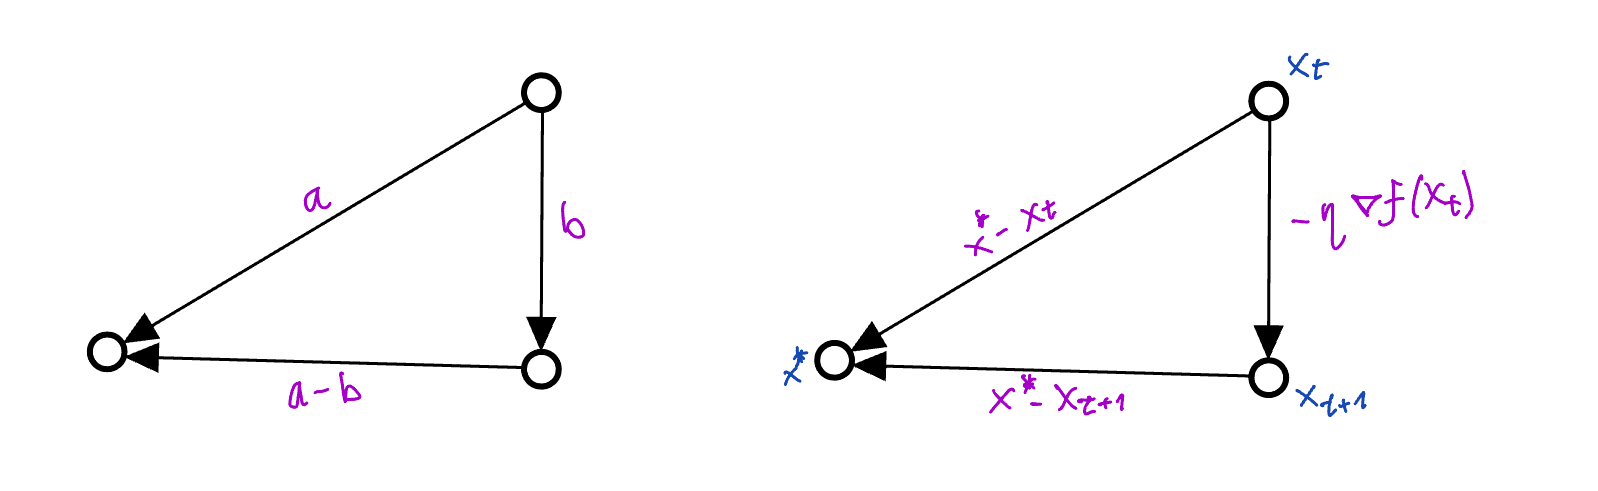
\includegraphics[width=0.8\textwidth]{Figs/vectors_triangle.jpeg}
    \caption{Gradient Descent}
\end{figure}

Then if we sum the above inequality from $t=1$ to $T$, we get:
\begin{align*}
    \sum_{t=1}^T ( f(x_t) - f(x^*) ) &\leq \frac{\|x_1 - x^*\|^2}{2 \eta} + \frac{\eta L^2}{2} T 
\end{align*}

In fact, this is a specific case of the Fundamental Inequality of Optimization. 

\begin{theorem}{Fundamental Inequality of Optimization (unconstrained version)} \\
    Suppose \( x_{t+1} = x_t - \eta g_t \) for all \( t \), where \( g_1, \ldots, g_T \in \mathbb{R}^d \) are arbitrary vectors. Then for all \( x^* \in \mathbb{R}^d \) it holds that
    \[
    \sum_{t=1}^T g_t \cdot (x_t - x^*) \leq \frac{\|x_1 - x^*\|^2}{2\eta} + \frac{\eta}{2} \sum_{t=1}^T \|g_t\|^2.
    \]
\end{theorem}
    
\begin{proof}{Fundamental Inequality of Optimization} \\
    The proof tracks \( \|x_t - x^*\|^2 \) as a ``potential''. First write
    \[
    \|x_{t+1} - x^*\|^2 = \|(x_t - x^*) - \eta g_t\|^2 = \|x_t - x^*\|^2 - 2\eta g_t \cdot (x_t - x^*) + \eta^2 \|g_t\|^2,
    \]
    that is,
    \[
    \|x_t - x^*\|^2 - \|x_{t+1} - x^*\|^2 = 2\eta g_t \cdot (x_t - x^*) - \eta^2 \|g_t\|^2.
    \]
    Summing over \( t = 1, \ldots, T \) and telescoping terms, we obtain
    \[
    \|x_1 - x^*\|^2 - \|x_{T+1} - x^*\|^2 = 2\eta \sum_{t=1}^T g_t \cdot (x_t - x^*) - \eta^2 \sum_{t=1}^T \|g_t\|^2.
    \]
    Organizing terms, we conclude:
    \[
    \sum_{t=1}^T g_t \cdot (x_t - x^*) \leq \frac{\|x_1 - x^*\|^2 - \|x_{T+1} - x^*\|^2}{2\eta} + \frac{\eta}{2} \sum_{t=1}^T \|g_t\|^2. \quad 
    \]
\end{proof}

\bigbreak


\todo{SGD , choosing eta} % Use the \todo command
    

% * * * * * * * * * * * * * * * * * * * * * * * * 
% * * * * * * * * * * * * * * * * * * * * * * * * 
% * * * * * * * * * * * * * * * * * * * * * * * * 
% * * * * * * * * * * * * * * * * * * * * * * * * 
% * * * * * * * * * * * * * * * * * * * * * * * * 
% * * * * * * * * * * * * * * * * * * * * * * * * 
% * * * * * * * * * * * * * * * * * * * * * * * * 
% * * * * * * * * * * * * * * * * * * * * * * * * 
% * * * * * * * * * * * * * * * * * * * * * * * * 
% * * * * * * * * * * * * * * * * * * * * * * * * 
% * * * * * * * * * * * * * * * * * * * * * * * * 
% * * * * * * * * * * * * * * * * * * * * * * * * 
% * * * * * * * * * * * * * * * * * * * * * * * * 
% * * * * * * * * * * * * * * * * * * * * * * * * 
% * * * * * * * * * * * * * * * * * * * * * * * * 
% * * * * * * * * * * * * * * * * * * * * * * * * 
% * * * * * * * * * * * * * * * * * * * * * * * * 
% * * * * * * * * * * * * * * * * * * * * * * * * 
% * * * * * * * * * * * * * * * * * * * * * * * * 

\chapter{The Second Miracle: Potential Based}

\section{Experts Problem}

At each time step, the player picks an action $I_t \in [n]$ (we have n experts) and the adversary picks a loss vector $l_t \in {0,1}^n$. 
The player incurs loss $l_t(I_t)$ and the goal is to minimize the regret:
\begin{equation}
    \text{Regret}_T(i) = \sum_{t=1}^T \left( l_t(I_t) - l_t(i) \right)
\end{equation}

We consider the case where in each time step the player chooses an action from a distribution $\vec{p}$ over the $n$ experts (a vector from the simplex):
\begin{equation*}
    \vec{p} \in \bigtriangleup_n = \{ \vec{p} \in \mathbb{R}_+^n : p_i \geq 0, \sum_{i=1}^n p_i = 1 \}
\end{equation*}

\subsubsection{Approach 1: Gradient Descent}
We can use gradient descent on $f_t(\vec{p}_t) = \vec{l_t} \cdot \vec{p}$, where $\vec{l_t}$ is the loss vector at time $t$.
It holds that $\nabla f_t(\vec{p}_t) = \vec{l_t}$. We can use the analysis of the gradient descent algorithm for gradient descent of convex functions varying in time.

Let $q \in \bigtriangleup_n$ be any distribution. Then we have:
\begin{align*}
    f_t(q) &\geq f_t(\vec{p}_t) + \nabla f_t(q) \cdot (q - \vec{p}_t) \Longrightarrow \\
    f_t(\vec{p}_t) - f_t(q) &\leq \nabla f_t(q) \cdot (\vec{p}_t - q) 
\end{align*}
Then:
\begin{align*}
    \| q - p_t \|^2 - \| q - p_{t+1} \|^2 &= - 2 \eta (q - p_t) \cdot \nabla f_t(p_t) - \eta^2 \| \nabla f_t(p_t) \|^2  \Longrightarrow \\
    f_t(\vec{p}_t) - f_t(q) &\leq \nabla f_t(q) \cdot (\vec{p}_t - q)  = \frac{1}{2\eta} \left( \| q - \vec{p}_t \|^2  - \| q - \vec{p}_{t+1} \|^2 \right) + \frac{\eta}{2} \| \nabla f_t(\vec{p}_t) \|^2 \Longrightarrow \\ 
    \sum_{t=1}^T \left( f_t(\vec{p}_t) - f_t(q) \right) &\leq \frac{1}{2\eta} \left( \| q - \vec{p}_1 \|^2 - \| q - \vec{p}_{T+1} \|^2 \right)+ \frac{\eta}{2} \sum_{t=1}^T \| \nabla f_t(\vec{p}_t) \|^2 \\
    &\leq \frac{1}{2\eta} \| q - \vec{p}_1 \|^2 + \frac{\eta}{2} \sum_{t=1}^T \| \nabla f_t(\vec{p}_t) \|^2 \\
    &\leq \frac{1}{\eta} + \frac{\eta}{2} T n  = \textbf{O} ( \sqrt{Tn} )
\end{align*}

We have used the facts that: 
\begin{itemize}
    \item Both $q$ and $\vec{p}_1$ are distributions, so $\| q - \vec{p}_1 \|^2 \leq 2$.
    \item $\| \nabla f_t(\vec{p}_t) \|^2 \leq n$ (as the loss vector is in ${0,1}^n$).
\end{itemize}

we can see that in this case, the rate of convergence DO depend on the dimension of the problem, in contrast to the non-varying case.
The fact that the rate of convergence DO NOT depend on the dimension of the problem in GD is one of the reasons why GD is so useful in practice.


\subsubsection{Approach 2: Multiplicative Weights Update (MWU)}
\todo {Approach 2: M} % Use the \todo command


\section{Mirror Descent}

Endow K with a Riemannian structure: $<\cdot, \cdot>_x$ for each $x \in K$. 
Before: 
\begin{equation}
    x_{t+1} = x_t - \eta \nabla f(x_t) \rightarrow f(x + dx) \approx f(x) + \nabla f(x) \cdot dx
\end{equation}

% * * * * * * * * * * * * * * * * * * * * * * * * 
% * * * * * * * * * * * * * * * * * * * * * * * * 
% * * * * * * * * * * * * * * * * * * * * * * * * 
% * * * * * * * * * * * * * * * * * * * * * * * * 
% * * * * * * * * * * * * * * * * * * * * * * * * 
% * * * * * * * * * * * * * * * * * * * * * * * * 
% * * * * * * * * * * * * * * * * * * * * * * * * 
% * * * * * * * * * * * * * * * * * * * * * * * * 
% * * * * * * * * * * * * * * * * * * * * * * * * 
% * * * * * * * * * * * * * * * * * * * * * * * * 
% * * * * * * * * * * * * * * * * * * * * * * * * 
% * * * * * * * * * * * * * * * * * * * * * * * * 
% * * * * * * * * * * * * * * * * * * * * * * * * 
% * * * * * * * * * * * * * * * * * * * * * * * * 
% * * * * * * * * * * * * * * * * * * * * * * * * 
% * * * * * * * * * * * * * * * * * * * * * * * * 
% * * * * * * * * * * * * * * * * * * * * * * * * 
% * * * * * * * * * * * * * * * * * * * * * * * * 
% * * * * * * * * * * * * * * * * * * * * * * * * 

\chapter{The Third Miracle: }

% * * * * * * * * * * * * * * * * * * * * * * * * 
% * * * * * * * * * * * * * * * * * * * * * * * * 
% * * * * * * * * * * * * * * * * * * * * * * * * 
% * * * * * * * * * * * * * * * * * * * * * * * * 
% * * * * * * * * * * * * * * * * * * * * * * * * 
% * * * * * * * * * * * * * * * * * * * * * * * * 
% * * * * * * * * * * * * * * * * * * * * * * * * 
% * * * * * * * * * * * * * * * * * * * * * * * * 
% * * * * * * * * * * * * * * * * * * * * * * * * 
% * * * * * * * * * * * * * * * * * * * * * * * * 
% * * * * * * * * * * * * * * * * * * * * * * * * 
% * * * * * * * * * * * * * * * * * * * * * * * * 
% * * * * * * * * * * * * * * * * * * * * * * * * 
% * * * * * * * * * * * * * * * * * * * * * * * * 
% * * * * * * * * * * * * * * * * * * * * * * * * 
% * * * * * * * * * * * * * * * * * * * * * * * * 
% * * * * * * * * * * * * * * * * * * * * * * * * 
% * * * * * * * * * * * * * * * * * * * * * * * * 
% * * * * * * * * * * * * * * * * * * * * * * * * 

\chapter{The Fourth Miracle: }

% * * * * * * * * * * * * * * * * * * * * * * * * 
% * * * * * * * * * * * * * * * * * * * * * * * * 
% * * * * * * * * * * * * * * * * * * * * * * * * 
% * * * * * * * * * * * * * * * * * * * * * * * * 
% * * * * * * * * * * * * * * * * * * * * * * * * 
% * * * * * * * * * * * * * * * * * * * * * * * * 
% * * * * * * * * * * * * * * * * * * * * * * * * 
% * * * * * * * * * * * * * * * * * * * * * * * * 
% * * * * * * * * * * * * * * * * * * * * * * * * 
% * * * * * * * * * * * * * * * * * * * * * * * * 
% * * * * * * * * * * * * * * * * * * * * * * * * 
% * * * * * * * * * * * * * * * * * * * * * * * * 
% * * * * * * * * * * * * * * * * * * * * * * * * 
% * * * * * * * * * * * * * * * * * * * * * * * * 
% * * * * * * * * * * * * * * * * * * * * * * * * 
% * * * * * * * * * * * * * * * * * * * * * * * * 
% * * * * * * * * * * * * * * * * * * * * * * * * 
% * * * * * * * * * * * * * * * * * * * * * * * * 
% * * * * * * * * * * * * * * * * * * * * * * * * 

\chapter{The Fifth Miracle: }

% * * * * * * * * * * * * * * * * * * * * * * * * 
% * * * * * * * * * * * * * * * * * * * * * * * * 
% * * * * * * * * * * * * * * * * * * * * * * * * 
% * * * * * * * * * * * * * * * * * * * * * * * * 
% * * * * * * * * * * * * * * * * * * * * * * * * 
% * * * * * * * * * * * * * * * * * * * * * * * * 
% * * * * * * * * * * * * * * * * * * * * * * * * 
% * * * * * * * * * * * * * * * * * * * * * * * * 
% * * * * * * * * * * * * * * * * * * * * * * * * 
% * * * * * * * * * * * * * * * * * * * * * * * * 
% * * * * * * * * * * * * * * * * * * * * * * * * 
% * * * * * * * * * * * * * * * * * * * * * * * * 
% * * * * * * * * * * * * * * * * * * * * * * * * 
% * * * * * * * * * * * * * * * * * * * * * * * * 
% * * * * * * * * * * * * * * * * * * * * * * * * 
% * * * * * * * * * * * * * * * * * * * * * * * * 
% * * * * * * * * * * * * * * * * * * * * * * * * 
% * * * * * * * * * * * * * * * * * * * * * * * * 
% * * * * * * * * * * * * * * * * * * * * * * * * 

\end{document}